\chapter{Testing}

\section{Test Plan}

\begin{landscape}
\subsection{Original Outline Plan}

\begin{center}
    \begin{tabular}{|p{2cm}|p{5cm}|p{5cm}|p{4cm}|}
        \hline
        \textbf{Test Series} & \textbf{Purpose of Test Series} & \textbf{Testing Strategy} & \textbf{Strategy Rationale}\\ \hline
1 & Test flow of control between the user interfaces & Top-down testing & A outline of the GUI will be developed and once working more modules will be added \\ \hline
       2 & To test validation of input data is performed correctly & Bottom-up testing & Components will be tested as they become available \\ \hline
3 & To test if the data is stored in its correct location & Black box testing & An output that the program produces will be examined for correctness and then the next output can be examined.\\ \hline
4 & To check information can be read from the database and read through the system & Bottom-up testing &  Components will be tested as they become available\\ \hline
5 & Check that the system cannot have unauthorised access & Unit testing & To test individual software components \\ \hline
6 & To check the finished system will fulfil the specifications &  Acceptance Testing & Performed by the client to check the system meets their requirements\\ \hline
7 & To test that the UI works effectively and certain shortcuts can be pressed & Black Box Testing & An output that the program produces will be examined for correctness and then the next output can be examined.\\ \hline
8 & Test algorithms to make sure that the output is correct & White Box Testing & Tests will be derived from knowledge of the program code \\ \hline

    \end{tabular}
\end{center}

\subsection{Changes to Outline Plan}

There were no changes made to my outline plan.

\begin{center}
    \begin{tabular}{|p{2cm}|p{5cm}|p{5cm}|p{4cm}|}
        \hline
        \textbf{Test Series} & \textbf{Purpose of Test Series} & \textbf{Testing Strategy} & \textbf{Strategy Rationale}\\ \hline
1 & Test flow of control between the user interfaces & Top-down testing & A outline of the GUI will be developed and once working more modules will be added \\ \hline
       2 & To test validation of input data is performed correctly & Bottom-up testing & Components will be tested as they become available \\ \hline
3 & To test if the data is stored in its correct location & Black box testing & An output that the program produces will be examined for correctness and then the next output can be examined.\\ \hline
4 & To check information can be read from the database and read through the system & Bottom-up testing &  Components will be tested as they become available\\ \hline
5 & Check that the system cannot have unauthorised access & Unit testing & To test individual software components \\ \hline
6 & To check the finished system will fulfil the specifications &  Acceptance Testing & Performed by the client to check the system meets their requirements\\ \hline
7 & To test that the UI works effectively and certain shortcuts can be pressed & Black Box Testing & An output that the program produces will be examined for correctness and then the next output can be examined.\\ \hline
8 & Test algorithms to make sure that the output is correct & White Box Testing & Tests will be derived from knowledge of the program code \\ \hline

    \end{tabular}
\end{center}

\subsection{Original Detailed Plan}

\begin{center}
    \begin{longtable}{|p{1.5cm}|p{2cm}|p{2.5cm}|p{4cm}|p{2cm}|p{2cm}|p{1cm}|p{1.7cm}|}
        \hline
        \textbf{Test Series} & \textbf{Purpose of Test} & \textbf{Test Description} & \textbf{Test Data} & \textbf{Test Data Type (Normal/ Erroneous/ Boundary)} & \textbf{Expected Result} & \textbf{Actual Result} & \textbf{Evidence}\\ \hline
1.01 & Test the manager login button on the select login page to ensure it works correctly  & This takes the user to the appropriate login screen & Click the Manager Login button & Normal & The manager login screen should be displayed && \\ \hline
1.02 & Test the staff login button on the select login page to ensure it works corrently & This takes the user to the appropriate login screen & Click the Staff Login button & Normal & The staff login screen should be displayed && \\ \hline
1.03 & Test the staff admin button on the select login page to ensure it works corrently & This takes the user to the appropriate login screen & Click the Admin Login button & Normal & The admin login screen should be displayed && \\ \hline
1.04 & Test the log in button on the manager login screen  & This takes the user to the appropriate main menu & Click the Log In button on the manager login screen & Normal & The manager main menu screen displayed && \\ \hline
1.05 & Test the log in button on the staff login screen  & This takes the user to the appropriate main menu & Click the Log In button on the staff login screen & Normal & The staff main menu screen displayed && \\ \hline
1.05 & Test the log in button on the admin login screen  & This takes the user to the appropriate main menu & Click the Log In button on the admin login screen & Normal & The admin main menu screen displayed && \\ \hline
1.06 & Test the forgot password button on the login screens & Takes the user to password recovery & Click the forgot password button & Normal & The password recovery form will be displayed && \\ \hline
1.07 & Test the submit button on the password recovery form & After the user enters form details they will click this to send it to IT staff & Click the submit button & Normal & An email will be sent to the IT staff (or the email specified) && \\ \hline
1.08 & Test the view department  button on the manager homepage & Will take the user to view their department information & Click the view department button & Normal & The layout will be switched to the staff database showing only people in their department && \\ \hline
1.09 & Test the view my information button on the manager homepage & Will take the user to view their own information & Click the view own information button& Normal  & The layout will be switched to the staff database showing only their own information && \\ \hline
1.10 & Test the cancel button on the change password screen & No changes will be saved & Click the cancel button & Normal & The window will close && \\ \hline
1.11 & Test the change button on the change password screen & Changes will be saved & Click the change button & Normal & The window will close and changes will be saved&& \\ \hline
1.12 & Test the cancel button on the report bug screen & Changes will not be saved & Click the cancel button & Normal & The window will close&& \\ \hline
1.13 & Test the submit button on the report bug screen & Changes will be saved and the form will be sent to IT staff & Click the submit button& Normal  & The window will close and an email will be sent to IT staff with all details (or the email specified) && \\ \hline
1.14 & Test the cancel button on the report errors screen & Changes will not be saved & Click the cancel button & Normal & The window will close&& \\ \hline
1.15 & Test the submit button on the report errors screen & Changes will be saved and the form will be sent to IT staff & Click the submit button& Normal  & The window will close and an email will be sent to IT staff with all details (or the email specified) && \\ \hline
1.16 & Test the open database button on the admin home screen & The open database screen should open & Click the open database button& Normal  & The window should switch layouts to the open database screen && \\ \hline
1.17 & Test the search for staff button on the admin home screen & The search staff screen should open & Click the search staff button& Normal  & The window should switch layouts to the search staff screen && \\ \hline
1.18 & Test the close button on the staff information (search staff screen) & The window will close  & Click the close button& Normal  & The window should close and return to the search screen && \\ \hline
1.19 & Test the edit database button on the open database screen & To test whether the edit buttons will shown up  & Click the edit database button& Normal  & Buttons to edit the data should show up && \\ \hline
1.20 & Test the edit button on the edit database screen & To test whether the edit buttons will open up a edit screen  & Click a edit button& Normal  & A new screen will appear allowing the user to enter information && \\ \hline
1.21 & Test the save changes button on the edit database input screen & To test whether the save changes button will save the changes made  & Click a save changes button& Normal  & The screen will close but changes will have applied && \\ \hline
1.22 & Test the add data button on the open database screen & To test whether screen to input data will show up  & Click the add data button& Normal  & The window to add data to the database will show up && \\ \hline
1.23 & Test the add data button on the data input screen & To test whether data will be added to the database  & Click the add data button& Normal  & The window will close and the data entered will have been added to the database && \\ \hline
1.24 & Test the remove data button on the open database screen & To test whether delete buttons will show up next to the records in the database  & Click the remove data button& Normal  & The delete buttons will show up next to each record && \\ \hline
1.25 & Test the delete buttons on the delete data screen & To test whether delete buttons will display a message  & Click a delete data button & Normal  & A warning sign should show up to confirm the user would like to remove the selected data && \\ \hline
1.26 & Test the no button on the delete data warning window & To test whether the no button will keep the data from being deleted  & Click the no data button & Normal  & The warning window will close and return to the previous screen. && \\ \hline
1.27 & Test the yes button on the delete data warning window & To test whether the yes button will delete the data selected  & Click the yes data button & Normal  & The warning window will close and return to the previous screen with the specified data deleted . && \\ \hline

1.28 & Test the Help menu (on Staff and Manager GUI) & To test whether a dropdown list of buttons will show up  & Click the help menu & Normal  & The menu should function correctly and display the "report bug" and "report incorrect information" buttons . && \\ \hline
1.29 & Test the Help menu buttons (on Staff and Manager GUI) & To test whether the buttons will work on the help menu  & Click the report bug and report incorrect information buttons & Normal  & The "report bug" should take the user to the report bug screen and "report incorrect information" should take the user to the report incorrect information screen . && \\ \hline

1.30 & Test the Account menu & To test whether a dropdown list of buttons will show up  & Click the account menu & Normal  & The menu should function correctly and display the "log out" and "change password" buttons . && \\ \hline
1.31 & Test the Account menu buttons & To test whether the buttons will work on the account menu  & Click the log out and change password buttons & Normal  & The "log out" should take the user back to the intitial login screen and "change password" should take the user to the change password screen . && \\ \hline

1.32 & Test the View menu (on Manager GUI)  & To test whether a dropdown list of buttons will show up  & Click the view menu & Normal  & The menu should function correctly and display the "department database" and "your information" buttons . && \\ \hline
1.33 & Test the View menu buttons (on Manager GUI) & To test whether the buttons will work on the view menu  & Click the department database and your information buttons & Normal  & The "department database" should take the user to the department database screen "your information" should take the staff database showing only your information . && \\ \hline

1.34 & Test the Database menu (on Admin GUI)  & To test whether a dropdown list of buttons will show up  & Click the Database menu & Normal  & The menu should function correctly and display "Staff", "Hardware", "Location" and "Department"  which all have secondary buttons to view, edit, add and remove data&& \\ \hline
1.35 & Test the Database menu buttons (on Admin GUI) & To test whether the buttons will work on the database menu coming off of  "Staff", "Hardware", "Location" and "Department"  & Click each button & Normal  & Each button will take the user to the specified database and either the normal view screen, edit screen, add data screen or remove data screen && \\ \hline

1.36 & Test the arrow buttons on the seach staff screen & To test whether the buttons next to each record will open a new window to view more information  & Click each button & Normal  & Any button should open up a screen to display more information about a staff member && \\ \hline

1.37 & Test the return to database view button on the open database screen & After Edit, Add or Remove is clicked the user may click this button to return to the viewing mode & Click return to database view button & Normal  & The layout will change to the normal view. && \\ \hline

1.38 & Test the back button on the admin interfaces & These buttons will take the user back to the home page & Click the return button & Normal  & The layout will change to the admin home page. && \\ \hline

2.1 & Test the dropdown boxes for department selection & To test whether the drop down boxes will function corrently on the open database and the search staff page. The options must actually open that database  & Click each button on the dropdown box & Normal  & Each button should open the database wanted && \\ \hline
2.2 & Test the dropdown boxes for data input windows (e.g. location and department) & To test whether the drop down boxes will function corrently when inputting data. The options must actually fill in the boxes once clicked  & Click each button on the dropdown box & Normal  & Each button should fill the box with the selection chosen && \\ \hline

2.3 & Test the calender works for date inputs & To test whether the calender will open when the icon is clicked. Once a date is selected it should automatically fill the box. & Click a date on the calender & Normal  & The date should be entered once a date on the calender is clicked in the following format DD/MM/YYYY && \\ \hline
2.4 & Verify that the username field has between 3 - 12 characters in it & The field cannot be blank, it has to have more than 3 characters but no more than 12. & Nothing \par \bigskip 30597 \par \bigskip JSmith21 \par \bigskip JordanSumerfield &Erroneous \par \bigskip  Normal \par \bigskip Normal \par \bigskip Erroneous & Error         \par \bigskip Valid              \par \bigskip Valid                 \par \bigskip Error && \\ \hline
2.5 & Verify that the password field has between 6 - 20 characters in it & The field cannot be blank, it has to have more than 6 characters but no more than 20. & Nothing \par password \par pA33WoRD \par cat  &Erroneous \par Normal \par Normal \par Erroneous & Error         \par Valid              \par Valid                 \par Error && \\ \hline
2.6 & Verify Email, Forename, Surname is entered in recover password fields & The fields cannot be blank and must have a '@' symbol in the email address. & John, Smith, J.com \par  \bigskip John, Smith, \par J@gmail.com \bigskip \par JJ, D, JJD@hotmail.com \par & Erroneous \par \bigskip Normal \par \bigskip \bigskip Normal &  \par Valid \par \bigskip Valid \par \bigskip \bigskip Valid&&\\ \hline
2.7 & Verify Email, Forename, Surname, Job Title, Date and Details of bug are entered in the report bug page & All fields must have some data in them before the submit  button is clicked & All fields filled out apart from Details of bug \par \bigskip All details filled out & Erroneous \par \bigskip \bigskip Normal & Error \par\bigskip \bigskip Valid && \\ \hline
2.8 & Verify Email, Forename, Surname and description are entered in the report errors page & All fields must have some data in them before the submit  button is clicked & All fields filled out apart from forename \par \bigskip All details filled out & Erroneous \par \bigskip \bigskip Normal & Error \par \bigskip \bigskip Valid && \\ \hline

3.01 & Verify the Staff details are entered into the Staff database using add data UI and conforms to validation rules& All information should be added to the required fields  & Staff information & Normal& Data is added to Staff table && \\ \hline
3.02 & Verify the Hardware details are entered into the Hardware database using add data UI and conforms to validation rules & All information should be added to the required fields  &Hardware information & Normal& Data is added to Hardware table && \\ \hline
3.03 & Verify the Location details are entered into the Location database using add data UI and conforms to validation rules & All information should be added to the required fields  &Location information & Normal& Data is added to Location table && \\ \hline
3.04 & Verify the Department details are entered into the Department database using add data UI and conforms to validation rules & All information should be added to the required fields  &Department information & Normal& Data is added to Department table && \\ \hline
3.05 & Verify the DeviceType details are entered into the DeviceType database using add data UI and conforms to validation rules & All information should be added to the required fields  &DeviceType information & Normal& Data is added to DeviceType table && \\ \hline
3.06 & Verify the HardwareMake details are entered into the HardwareMake database using add data UI and conforms to validation rules & All information should be added to the required fields  &HardwareMake information & Normal& Data is added to HardwareMake table && \\ \hline
3.07 & Verify the HardwareModel details are entered into the HardwareModel database using add data UI and conforms to validation rules & All information should be added to the required fields  &HardwareModel information & Normal& Data is added to HardwareModel table && \\ \hline
3.08 & Verify the Staff's Hardware details with purchase date are entered into the StaffHardware database using add data UI and conforms to validation rules & All information should be added to the required fields  &StaffHardware information & Normal& Data is added to StaffHardware table && \\ \hline
3.09 & Verify the DepartmentLocation details with purchase date are entered into the DepartmentLocation database using add data UI and conforms to validation rules & All information should be added to the required fields  &DepartmentLocation information & Normal& Data is added to DepartmentLocation table && \\ \hline
3.10 & Verify that user can update Staff details in the database using UI & When the Update Database button is clicked, the user should be able to edit cells in the current table. This should change the database file if the save changes button is clicked. & Blank \par \bigskip John & Erroneous \par \bigskip Normal & Data should appear in the database && \\ \hline
3.11 & Verify that user can update Hardware details in the database using UI & When the Update Database button is clicked, the user should be able to edit cells in the current table. This should change the database file if the save changes button is clicked. & Blank \par \bigskip £100 & Erroneous \par \bigskip Normal & Data should appear in the database && \\ \hline
3.12 & Verify that user can update Location details in the database using UI & When the Update Database button is clicked, the user should be able to edit cells in the current table. This should change the database file if the save changes button is clicked. & Blank \par \bigskip Orwell & Erroneous \par \bigskip Normal & Data should appear in the database && \\ \hline
3.13 & Verify that user can update Department details in the database using UI & When the Update Database button is clicked, the user should be able to edit cells in the current table. This should change the database file if the save changes button is clicked. & Blank \par \bigskip Financing & Erroneous \par \bigskip Normal & Data should appear in the database && \\ \hline
3.14 & Verify that user can update DeviceType details in the database using UI & When the Update Database button is clicked, the user should be able to edit cells in the current table. This should change the database file if the save changes button is clicked. & Blank \par \bigskip Phone & Erroneous \par \bigskip Normal & Data should appear in the database && \\ \hline
3.15 & Verify that user can update HardwareMake details in the database using UI & When the Update Database button is clicked, the user should be able to edit cells in the current table. This should change the database file if the save changes button is clicked. & Blank \par \bigskip iPhone & Erroneous \par \bigskip Normal & Data should appear in the database && \\ \hline
3.16 & Verify that user can update HardwareModel details in the database using UI & When the Update Database button is clicked, the user should be able to edit cells in the current table. This should change the database file if the save changes button is clicked. & Blank \par \bigskip 4S & Erroneous \par \bigskip Normal & Data should appear in the database && \\ \hline
3.17 & Verify that user can update Staff's Hardware details in the database using UI & When the Update Database button is clicked, the user should be able to edit cells in the current table. This should change the database file if the save changes button is clicked. & Blank \par \bigskip 13/12/2015 & Erroneous \par \bigskip Normal & Data should appear in the database && \\ \hline
3.18 & Verify that user can update DepartmentLocation details in the database using UI & When the Update Database button is clicked, the user should be able to edit cells in the current table. This should change the database file if the save changes button is clicked. & Blank \par \bigskip 1 & Erroneous \par \bigskip Normal & Data should appear in the database && \\ \hline


4 & Verify each table can be read by clicking the dropdown box and selecting the database wanted & Each table should be able to be clicked and be viewed in a table format&Data from the following tables: \par Staff \par Hardware \par Location \par Department \par DeviceType \par HardwareMake \par HardwareModel \par StaffHardware \par DepartmentLocation & Normal& The table will be shown and will match information in the database && \\ \hline

5.1 & Check that staff members cannot log in to managers or admins interfaces & Staff should not be able to use their login to access the admin interface or the manager interface, only their own. & Staff login details & Erroneous & The system will say incorrect login details && \\ \hline
5.2 & Check that managers cannot log in to staff or admins interfaces & managers should not be able to use their login to access the admin interface or the staff interface, only their own. & managers login details & Erroneous & The system will say incorrect login details && \\ \hline
5.2 & Check that admins cannot log in to staff or managers interfaces & admins should not be able to use their login to access the manager interface or the staff interface, only their own. & admins login details & Erroneous & The system will say incorrect login details && \\ \hline

6 & Verify the program fulfils all the specifications & The program should meet the clients specification and the goals proposed in the Analysis stage & Run through the program testing every aspect with correct and incorrect data to insure all the objectives are met & Normal &The program should fulfil all specifications and objectives && \\ \hline

7.1 & Allow the enter button to be pressed on the login window instead of using the push button & To test if the enter button will work as an alternative & press the enter button while on the login screen & Normal & The layout will switch to the appropriate main menu && \\ \hline
7.2 & Allow the escape button to be used to close the calendar widget & The user should be able to use escape instead of pressing the cross to close the window & Press ESC when calendar is opened from add data screen & Normal & The calendar should close with TAB && \\ \hline
7.3  & Allow the TAB button to be pressed on all data inputs with line edits & The user will be able to switch line edits using TAB & Press TAB on any data input & Normal & Should be able to switch line edits with tab && \\ \hline
7.4 & Login screen should be a fixed size & The user should not be able to resize the login window & Try to resize the window & Normal & The window should not allow itself to be resized && \\ \hline
7.5 & Clicking any blank space on an open window should not affect the program & Clicking on any area of a window with no functionality should not give any errors & Click anywhere on each window & Normal & Nothing should happen && \\ \hline
7.6 & User should not be able to click away from a dialog box & The user should not be able to click away from the Add Data dialog box without pressing the cross or the cancel/save changes button & Try to click off the dialog box & Normal & Window should stay raised and centralised && \\ \hline

8.1 & Verify that search function works correctly & Enter text into any search function on the program should return specified information back & -Enter some text into the search bar- & Normal & Returns results for the specified search && \\ \hline
8.2 & Verify new password overwrites old password when changed & The old password should not work if a new password is set & Try old password on login & Normal & Error && \\ \hline
8.3 & Verify that Managers and other Staff cannot change any data in the table & No unauthorised staff should be able to edit anything in the table & Try to change data in tables using Manager and Staff logins & Normal & Error && \\ \hline

    \end{longtable}
\end{center}


\subsection{Changes to Detailed Plan}

Changes made are shown in light grey. The tests that have been removed are shown in darker grey.

\begin{center}
    \begin{longtable}{|p{1.5cm}|p{2cm}|p{2.5cm}|p{2cm}|p{2cm}|p{2cm}|p{3cm}|p{1.7cm}|}
        \hline
        \textbf{Test Series} & \textbf{Purpose of Test} & \textbf{Test Description} & \textbf{Test Data} & \textbf{Test Data Type (Normal/ Erroneous/ Boundary)} & \textbf{Expected Result/reason for removal} & \textbf{Actual Result} & \textbf{Evidence}\\ \hline
\rowcolor{gray}1.01 & Test the manager login button on the select login page to ensure it works correctly  & This takes the user to the appropriate login screen & Click the Manager Login button & Normal & Page removed, all staff use one login screen now. & & \\ \hline
\rowcolor{gray}1.02 & Test the staff login button on the select login page to ensure it works corrently & This takes the user to the appropriate login screen & Click the Staff Login button & Normal &  Page removed, all staff use one login screen now. && \\ \hline
\rowcolor{gray}1.03 & Test the staff admin button on the select login page to ensure it works corrently & This takes the user to the appropriate login screen & Click the Admin Login button & Normal &  Page removed, all staff use one login screen now. && \\ \hline
\rowcolor{gray}1.04 & Test the log in button on the manager login screen  & This takes the user to the appropriate main menu & Click the Log In button on the manager login screen & Normal &  Page removed, all staff use one login screen now.&& \\ \hline
\rowcolor{gray}1.05 & Test the log in button on the staff login screen  & This takes the user to the appropriate main menu & Click the Log In button on the staff login screen & Normal &  Page removed, all staff use one login screen now.&& \\ \hline
\rowcolor{gray}1.05 & Test the log in button on the admin login screen  & This takes the user to the appropriate main menu & Click the Log In button on the admin login screen & Normal &  Page removed, all staff use one login screen now. && \\ \hline
\rowcolor{lightgray}1.02 & Test the log in button using admin details on the login screen  & This takes the user to the appropriate main menu & Click the Log In button on the login screen & Normal &  The appropriate interface should be displayed.&The admin inferace was displayed & Login Screen: \ref{fig:LoginScreen} and Admin Interface:  \ref{fig:AdminInterfaceLogin} on page \pageref{fig:LoginScreen} \\ \hline
\rowcolor{lightgray}1.03 & Test the log in button using manager details on the login screen  & This takes the user to the appropriate main menu & Click the Log In button on the login screen & Normal &  The appropriate interface should be displayed.& The manager interface was displayed & Manager Interface:  \ref{fig:ManagerInterfaceLogin}  \\ \hline
\rowcolor{lightgray}1.04 & Test the log in button using staff details on the login screen  & This takes the user to the appropriate main menu & Click the Log In button on the login screen & Normal &  The appropriate interface should be displayed.& The staff interface was displayed & Staff Interface:  \ref{fig:StaffInterfaceLogin}  \\ \hline
\rowcolor{lightgray}1.05 & Test the cancel button on the fogotten password interface & Closes password recovery & Click the cancel button & Normal & The password recovery will close & Password recovery window closed as expected &  \\ \hline
1.06 & Test the forgot password button on the login screen & Takes the user to password recovery & Click the forgot password button & Normal & The password recovery form will be displayed & The password recovery is displayed as expected& \ref{fig:ForgotPassword}  \\ \hline
1.07 & Test the submit button on the password recovery form & After the user enters form details they will click this to send it to IT staff & Click the submit button & Normal & An email will be sent to the IT staff (or the email specified) & The data was added to the database as expected &\ref{fig:SubmitPassword} \\ \hline
1.08 & Test the department information button on the manager homepage & Will take the user to view their department information & Click the view department button & Normal & The layout will be switched to the staff database showing only people in their department & The interface was changed as expected&  \ref {fig:DepartmentInformation}   \\ \hline

1.09 & Test the my information button on the manager homepage & Will take the user to view their own information & Click the view own information button& Normal  & The layout will be switched to the staff database showing only their own information &The interface was changed as expected&   \ref {fig:MyInformation} \\ \hline
1.10 & Test the cancel button on the change password screen & No changes will be saved & Click the cancel button & Normal & The window will close & Window closed as expected&  \\ \hline
1.11 & Test the change button on the change password screen & Changes will be saved & Click the change button & Normal & The window will close and changes will be saved&Password was changed as expected& \ref{fig:ChangePasswordWindow}\\ \hline
1.12 & Test the cancel button on the report bug screen & Changes will not be saved & Click the cancel button & Normal & The window will close&Window closed as expected& \\ \hline
1.13 & Test the submit button on the report bug screen & Changes will be saved and the form will be sent to IT staff & Click the submit button& Normal  & The window will close and an email will be sent to IT staff with all details (or the email specified) &Email received as expected and window closed &  \ref {fig:SubmitBugTest} \\ \hline
1.14 & Test the cancel button on the report errors screen & Changes will not be saved & Click the cancel button & Normal & The window will close& Window closed as expected& \\ \hline
1.15 & Test the submit button on the report errors screen & Changes will be saved and the form will be sent to IT staff & Click the submit button& Normal  & The window will close and an email will be sent to IT staff with all details (or the email specified) &Email received as expected and window closed & \ref {fig:SubmitErrorReport} \\ \hline
1.16 & Test the open database button on the admin home screen & The open database screen should open & Click the open database button& Normal  & The window should switch layouts to the open database screen &Open database screen opened as expected&\ref {fig:OpenDatabaseInterfaceBF} \\ \hline
1.17 & Test the search for staff button on the admin home screen & The search staff screen should open & Click the search staff button& Normal  & The window should switch layouts to the search staff screen & Search screen opened as expected&\ref {fig:SearchStaffInterfaceBF}  \\ \hline
\rowcolor{gray}1.18 & Test the close button on the staff information (search staff screen) & The window will close  & Click the close button& Normal  &The user has no close button, instead will click the window 'X' && \\ \hline
\rowcolor{gray}1.19 & Test the edit database button on the open database screen & To test whether the edit buttons will shown up  & Click the edit database button& Normal  & This design has been replaced. Buttons to Add,Edit,Remove will stay visible && \\ \hline
\rowcolor{gray}1.20 & Test the edit button on the edit database screen & To test whether the edit buttons will open up a edit screen  & Click a edit button& Normal  & This design has been replaced. User can now simply click a field in the table to overwrite it && \\ \hline
\rowcolor{lightgray}1.18 & Test the open database button on the open database screen   & Test that after the button is clicked a file browser will appear allowing the database to be chosen &Click the open database button and select the correct file & Normal &  The program should load the database into the table& Database opened as expected& \ref {fig:OpenDatabaseFileBefore} \\ \hline
\rowcolor{lightgray}1.19 & Test the edit button on the open database screen  & Test that after the button is clicked the table fields can be edited &Click a edit button and enter information & Normal & The program should allow the input of data.& Data can be edited as expected&  \ref {fig:EditDataBtn}\\ \hline
\rowcolor{lightgray}1.20 & Test the cancel button on the edit database input screen   & Test that after the button is clicked the changes will not be saved &Click the cancel button & Normal &   The information will go back to being ineditable but changes will not have applied& Changes did not save and went back to being ineditable & \ref {fig:CancelBtn} \\ \hline
1.21 & Test the save changes button on the edit database input screen & To test whether the save changes button will save the changes made  & Click a save changes button& Normal  & The information will go back to being ineditable but changes will have applied & Changes applied as expected & \ref {fig:SaveChanges} \\ \hline
1.22 & Test the add data button on the open database screen & To test whether screen to input data will show up  & Click the add data button& Normal  & The window to add data to the database will show up & Add data window appeared as expected&  \ref {fig:AddDataWindow} \\ \hline
1.23 & Test the add data button on the data input screen & To test whether data will be added to the database  & Click the add data button& Normal  & The window will close and the data entered will have been added to the database & Data added to database and table as expected&  \ref {fig:AddDataDataExample} \\ \hline
1.24 & Test the remove data button on the open database screen & To test whether delete buttons will show up next to the records in the database  & Click the remove data button& Normal  & The delete buttons will show up next to each record & Delete buttons showed as expected &\ref {fig:RemoveDataButtons} \\ \hline
1.25 & Test the delete buttons on the delete data screen & To test whether delete buttons will display a message  & Click a delete data button & Normal  & A warning sign should show up to confirm the user would like to remove the selected data & Data deletion warning message showed as expected  & \\ \hline
1.26 & Test the no button on the delete data warning window & To test whether the no button will keep the data from being deleted  & Click the no data button & Normal  & The warning window will close and return to the previous screen. & Window closed and no data was removed&\ref {fig:NoButton} \\ \hline
1.27 & Test the yes button on the delete data warning window & To test whether the yes button will delete the data selected  & Click the yes data button & Normal  & The warning window will close and return to the previous screen with the specified data deleted . &Window closed and data was removed&\ref {fig:YesBtn} \\ \hline

1.28 & Test the Help menu (on Staff and Manager GUI) & To test whether a dropdown list of buttons will show up  & Click the help menu & Normal  & The menu should function correctly and display the "report bug" and "report incorrect information" buttons . & Help menu works as expected &\ref {fig:HelpMenu} \\ \hline
1.29 & Test the Help menu buttons (on Staff and Manager GUI) & To test whether the buttons will work on the help menu  & Click the report bug and report incorrect information buttons & Normal  & The "report bug" should take the user to the report bug screen and "report incorrect information" should take the user to the report incorrect information screen . &Buttons worked as expected& \\ \hline

1.30 & Test the Account menu & To test whether a dropdown list of buttons will show up  & Click the account menu & Normal  & The menu should function correctly and display the "log out" and "change password" buttons . &Account menu works as expected&\ref {fig:AccountMenu} \\ \hline
1.31 & Test the Account menu buttons & To test whether the buttons will work on the account menu  & Click the log out and change password buttons & Normal  & The "log out" should take the user back to the intitial login screen and "change password" should take the user to the change password screen . &Buttons worked as expected & \\ \hline

1.32 & Test the View menu (on Manager GUI)  & To test whether a dropdown list of buttons will show up  & Click the view menu & Normal  & The menu should function correctly and display the "department database" and "your information" buttons . & View menu works as expected& \ref {fig:ViewMenu} \\ \hline
1.33 & Test the View menu buttons (on Manager GUI) & To test whether the buttons will work on the view menu  & Click the department database and your information buttons & Normal  & The "department database" should take the user to the department database screen "your information" should take the staff database showing only your information . &Buttons worked as expected& \\ \hline

\rowcolor{gray}1.34 & Test the Database menu (on Admin GUI)  & To test whether a dropdown list of buttons will show up  & Click the Database menu & Normal  & This menu has been remove since it is unnecessary&& \\ \hline
\rowcolor{gray}1.35 & Test the Database menu buttons (on Admin GUI) & To test whether the buttons will work on the database menu coming off of  "Staff", "Hardware", "Location" and "Department"  & Click each button & Normal  &  This menu has been remove since it is unnecessary && \\ \hline

\rowcolor{gray}1.36 & Test the arrow buttons on the seach staff screen & To test whether the buttons next to each record will open a new window to view more information  & Click each button & Normal  & The arrows have been added to buttons, the user can now click anywhere on the button to open the window && \\ \hline
\rowcolor{lightgray}1.36 & Test the buttons on the seach staff screen & To test whether the buttons will open a new window to view more information  & Click each button & Normal  & Each button should open more information on the staff member specified& Buttons worked as expected& \ref {fig:SearchStaffButtons}\\ \hline

\rowcolor{gray}1.37 & Test the return to database view button on the open database screen & After Edit, Add or Remove is clicked the user may click this button to return to the viewing mode & Click return to database view button & Normal  & This design has been replaced. Buttons to Add,Edit,Remove will stay visible && \\ \hline

1.38 & Test the back button on the admin interfaces & These buttons will take the user back to the home page & Click the return button & Normal  & The layout will change to the admin home page. & Back buttons work as expected& \\ \hline
\rowcolor{lightgray}1.39 & Test the generate graph toolbar button & A hardware graph should be generated in a new window & Click the toolbar button & Normal  & A new window will open with the graph displayed & Button generates graph as expected& \ref {fig:GraphBtn} \\ \hline
\rowcolor{lightgray}1.40 & Test the create user accounts toolbar button & A new window should appear allowing user account creation & Click the toolbar button & Normal  & A new window will open with account creation &Button opens create accounts window as expected &\ref {fig:AddAccountsBtn} \\ \hline
\rowcolor{lightgray}1.41 & Test the create accounts button on create user accounts layout & The line edits should fill depending on the entered informationl after the button is pressed & Click the create account button & Normal  & Line edits should be filled with information & Button works as expected & \ref {fig:AddAccountDetails}\\ \hline
\rowcolor{lightgray}1.42 & Test the add account button on create user accounts layout & Account information should be added to the database & Click the add account button & Normal  &User account should be working &Data added to database as expected& \\ \hline

2.1 & Test the dropdown boxes for department selection & To test whether the drop down boxes will function corrently on the open database and the search staff page. The options must actually open that database  & Click each button on the dropdown box & Normal  & Each button should open the database wanted & Dropdown box works as expected& \ref {fig:ComboBoxHardware} \\ \hline
2.2 & Test the dropdown boxes for data input windows (e.g. location and department) & To test whether the drop down boxes will function corrently when inputting data. The options must actually fill in the boxes once clicked  & Click each button on the dropdown box & Normal  & Each button should fill the box with the selection chosen &Dropdown boxes works as expected& \\ \hline

2.3 & Test the calender works for date inputs & To test whether the calender will open when the icon is clicked. Once a date is selected it should automatically fill the box. & Click a date on the calender & Normal  & The date should be entered once a date on the calender is clicked in the following format DD/MM/YYYY &Calendar works as expected&  \ref {fig:Calendar} \\ \hline
\rowcolor{gray}2.4 & Verify that the username field has between 3 - 12 characters in it & The field cannot be blank, it has to have more than 3 characters but no more than 12. & Nothing \par \bigskip 30597 \par \bigskip JSmith21 \par \bigskip JordanSumerfield &Erroneous \par \bigskip  Normal \par \bigskip Normal \par \bigskip Erroneous &The validation has been removed && \\ \hline
\rowcolor{gray}2.5 & Verify that the password field has between 6 - 20 characters in it & The field cannot be blank, it has to have more than 6 characters but no more than 20. & Nothing \par password \par pA33WoRD \par cat  &Erroneous \par Normal \par Normal \par Erroneous &The validation has been removed && \\ \hline
2.6 & Verify Email, Forename, Surname is entered in recover password fields & The fields cannot be blank and must have a '@' symbol in the email address. & John, Smith, J.com \par  \bigskip John, Smith, \par J@gmail.com \bigskip \par JJ, D, JJD@hotmail.com \par & Erroneous \par \bigskip Normal \par \bigskip \bigskip Normal &  \par Valid \par \bigskip Valid \par \bigskip \bigskip Valid&Errors were given where required. Everything worked as expected.& \\ \hline
2.7 & Verify Email, Forename, Surname, Job Title, Date and Details of bug are entered in the report bug page & All fields must have some data in them before the submit  button is clicked & All fields filled out apart from Details of bug \par \bigskip All details filled out & Erroneous \par \bigskip \bigskip Normal & Error \par\bigskip \bigskip Valid &Errors were given where required. Everything worked as expected.&\ref {fig:ReportBugValidation} \\ \hline
2.8 & Verify Email, Forename, Surname and description are entered in the report errors page & All fields must have some data in them before the submit  button is clicked & All fields filled out apart from forename \par \bigskip All details filled out & Erroneous \par \bigskip \bigskip Normal & Error \par \bigskip \bigskip Valid &Errors were given where required. Everything worked as expected.&\ref {fig:ReportErrorValidation}  \\ \hline
\rowcolor{lightgray}2.9 & Test to see if warning dialog box will appear when the incorrect file is opened from the open database screen & If the incorrect file is opened a warning dialog should appear to disallow the tables to be shown & Click on the wrong file & Normal &Warning dialog box should appear &Dailog box appeared as expected& \ref {fig:IncorrectFile}  \\ \hline
\rowcolor{lightgray}2.10& Test to see if warning dialog box will appear when a primary key referenced somewhere else is being deleted & If the primary key cannot be deleted a warning dialog should appear to disallow the user to delete it & Delete a primary key referenced in another table & Normal &Warning dialog box should appear &Dailog box appeared as expected& \ref{fig:DialogNoClickAway} \\ \hline


3.01 & Verify the Staff details are entered into the Staff database using add data UI and conforms to validation rules& All information should be added to the required fields  & Staff information & Normal& Data is added to Staff table &Works as expected& \\ \hline
3.02 & Verify the Hardware details are entered into the Hardware database using add data UI and conforms to validation rules & All information should be added to the required fields  &Hardware information & Normal& Data is added to Hardware table &Works as expected& \\ \hline
3.03 & Verify the Location details are entered into the Location database using add data UI and conforms to validation rules & All information should be added to the required fields  &Location information & Normal& Data is added to Location table &Works as expected& \\ \hline
3.04 & Verify the Department details are entered into the Department database using add data UI and conforms to validation rules & All information should be added to the required fields  &Department information & Normal& Data is added to Department table &Works as expected& \\ \hline
3.05 & Verify the DeviceType details are entered into the DeviceType database using add data UI and conforms to validation rules & All information should be added to the required fields  &DeviceType information & Normal& Data is added to DeviceType table &Works as expected&\ref {fig:Dev} \\ \hline
3.06 & Verify the HardwareMake details are entered into the HardwareMake database using add data UI and conforms to validation rules & All information should be added to the required fields  &HardwareMake information & Normal& Data is added to HardwareMake table &Works as expected& \\ \hline
3.07 & Verify the HardwareModel details are entered into the HardwareModel database using add data UI and conforms to validation rules & All information should be added to the required fields  &HardwareModel information & Normal& Data is added to HardwareModel table &Works as expected& \\ \hline
3.08 & Verify the Staff's Hardware details with purchase date are entered into the StaffHardware database using add data UI and conforms to validation rules & All information should be added to the required fields  &StaffHardware information & Normal& Data is added to StaffHardware table &Works as expected& \\ \hline
\rowcolor{gray}3.09 & Verify the DepartmentLocation details with purchase date are entered into the DepartmentLocation database using add data UI and conforms to validation rules & All information should be added to the required fields  &DepartmentLocation information & Normal&The department location table has been removed since it was unnecessary && \\ \hline
3.10 & Verify that user can update Staff details in the database using UI & When the Update Database button is clicked, the user should be able to edit cells in the current table. This should change the database file if the save changes button is clicked. & Blank \par \bigskip John & Erroneous \par \bigskip Normal & Data should appear in the database &User can update information as expected& \\ \hline
3.11 & Verify that user can update Hardware details in the database using UI & When the Update Database button is clicked, the user should be able to edit cells in the current table. This should change the database file if the save changes button is clicked. & Blank \par \bigskip £100 & Erroneous \par \bigskip Normal & Data should appear in the database &User can update information as expected& \\ \hline
3.12 & Verify that user can update Location details in the database using UI & When the Update Database button is clicked, the user should be able to edit cells in the current table. This should change the database file if the save changes button is clicked. & Blank \par \bigskip Orwell & Erroneous \par \bigskip Normal & Data should appear in the database &User can update information as expected& \\ \hline
3.13 & Verify that user can update Department details in the database using UI & When the Update Database button is clicked, the user should be able to edit cells in the current table. This should change the database file if the save changes button is clicked. & Blank \par \bigskip Financing & Erroneous \par \bigskip Normal & Data should appear in the database &User can update information as expected& \\ \hline
3.14 & Verify that user can update DeviceType details in the database using UI & When the Update Database button is clicked, the user should be able to edit cells in the current table. This should change the database file if the save changes button is clicked. & Blank \par \bigskip Phone & Erroneous \par \bigskip Normal & Data should appear in the database &User can update information as expected& \\ \hline
3.15 & Verify that user can update HardwareMake details in the database using UI & When the Update Database button is clicked, the user should be able to edit cells in the current table. This should change the database file if the save changes button is clicked. & Blank \par \bigskip iPhone & Erroneous \par \bigskip Normal & Data should appear in the database &User can update information as expected& \\ \hline
3.16 & Verify that user can update HardwareModel details in the database using UI & When the Update Database button is clicked, the user should be able to edit cells in the current table. This should change the database file if the save changes button is clicked. & Blank \par \bigskip 4S & Erroneous \par \bigskip Normal & Data should appear in the database &User can update information as expected& \\ \hline
3.17 & Verify that user can update Staff's Hardware details in the database using UI & When the Update Database button is clicked, the user should be able to edit cells in the current table. This should change the database file if the save changes button is clicked. & Blank \par \bigskip 13/12/2015 & Erroneous \par \bigskip Normal & Data should appear in the database &User can update information as expected& \\ \hline
\rowcolor{gray}3.18 & Verify that user can update DepartmentLocation details in the database using UI & When the Update Database button is clicked, the user should be able to edit cells in the current table. This should change the database file if the save changes button is clicked. & Blank \par \bigskip 1 & Erroneous \par \bigskip Normal & The department location table has been removed since it was unnecessary&& \\ \hline
\rowcolor{lightgray}3.18 & Check that emails sent from the program appear in IT staff inbox (or test inbox) & When a user submits data using email  it should appear in the specified email inbox & Submit emails from Report Bug, Report Incorrect Information, forgotten user accounts or allow the program to send an automated warranty email & Normal &The correct subject and body should appear in the email &All emails working as expected&\ref {fig:EmailExpiredHardware} \\ \hline


4 & Verify each table can be read by clicking the dropdown box and selecting the database wanted & Each table should be able to be clicked and be viewed in a table format&Data from the following tables: \par Staff \par Hardware \par Location \par Department \par DeviceType \par HardwareMake \par HardwareModel \par StaffHardware \par DepartmentLocation & Normal& The table will be shown and will match information in the database &Works as expected& \ref {fig:ComboBoxHardware}\\ \hline

5.1 & Check that staff members cannot log in to managers or admins interfaces & Staff should not be able to use their login to access the admin interface or the manager interface, only their own. & Staff login details & Erroneous & The system will say incorrect login details & Works as expected& \\ \hline
5.2 & Check that managers cannot log in to staff or admins interfaces & managers should not be able to use their login to access the admin interface or the staff interface, only their own. & managers login details & Erroneous & The system will say incorrect login details & Works as expected& \\ \hline
5.2 & Check that admins cannot log in to staff or managers interfaces & admins should not be able to use their login to access the manager interface or the staff interface, only their own. & admins login details & Erroneous & The system will say incorrect login details & Works as expected& \\ \hline

6 & Verify the program fulfils all the specifications & The program should meet the clients specification and the goals proposed in the Analysis stage & Run through the program testing every aspect with correct and incorrect data to insure all the objectives are met & Normal &The program should fulfil all specifications and objectives &Not all of the specifications were met in time including and most importantly making the database online so multiple people can access it. This challenege was beyond what I was capable of in the time space given. However to program can replace the current spreadsheet but will need further work.& \\ \hline

7.1 & Allow the enter button to be pressed on the login window instead of using the push button & To test if the enter button will work as an alternative & press the enter button while on the login screen & Normal & The layout will switch to the appropriate main menu &Shortcut works as expected& \\ \hline
7.2 & Allow the escape button to be used to close the calendar widget & The user should be able to use escape instead of pressing the cross to close the window & Press ESC when calendar is opened from add data screen & Normal & The calendar should close with ESC &Shortcut works but an error is displayed in the consol. This can be ignored but is not ideal.& \\ \hline
7.3  & Allow the TAB button to be pressed on all data inputs with line edits & The user will be able to switch line edits using TAB & Press TAB on any data input & Normal & Should be able to switch line edits with tab &Shortcut works as expected& \\ \hline
7.4 & Login screen should be a fixed size & The user should not be able to resize the login window & Try to resize the window & Normal & The window should not allow itself to be resized &Window is a fixed size& \\ \hline
7.5 & Clicking any blank space on an open window should not affect the program & Clicking on any area of a window with no functionality should not give any errors & Click anywhere on each window & Normal & Nothing should happen &As expected& \\ \hline
7.6 & User should not be able to click away from a dialog box & The user should not be able to click away from the Add Data dialog box without pressing the cross or the cancel/save changes button & Try to click off the dialog box & Normal & Window should stay raised and centralised &Dialogs work as expected& \\ \hline
\rowcolor{lightgray}7.7 & Allow CTRL-C to be pressed on all  interfaces to show change password window & To test if the CTRL-C will work as an alternative to pressing the menu button & press CTRL-C  while on each window of the interfaces & Normal & The change password window should show up &Shortcut works as expected& \\ \hline
\rowcolor{lightgray}7.8 & Allow CTRL-W to be pressed on all interfaces to close program & To test if the CTRL-W will work as an alternative to pressing the menu button & press CTRL-W while on each window of the interfaces & Normal & The program should close &Shortcut works as expected& \\ \hline
\rowcolor{lightgray}7.9 & Allow CTRL-S to be pressed on the open database layout when information has been changed to save changes& To test if the CTRL-S will work as an alternative to pressing the push button & press CTRL-S when information has been changed & Normal & The information will go back to being ineditable but changes will have applied  &Shortcut works as expected& \\ \hline
\rowcolor{lightgray}7.10 & Allow CTRL-X to be pressed on the open database layout when information has been changed to cancel changes & To test if the CTRL-X will work as an alternative to pressing the push button & press CTRL-X when information has been changed & Normal & The information will go back to being ineditable and changes will not have applied  &Shortcut works as expected& \\ \hline
\rowcolor{lightgray}7.11& Allow F1 to be pressed on the manager interface to switch to Department Information  & To test if the F1 will work as an alternative to pressing the push button & press F1 on any layout of manager interface & Normal & The department information layout will be shown  &Shortcut works as expected& \ref {fig:DepartmentInformationButton}\\ \hline
\rowcolor{lightgray}7.12 & Allow F2 to be pressed on the manager interface to switch to My Information  & To test if the F1 will work as an alternative to pressing the push button & press F1 on any layout of manager interface & Normal & The My Infomation layout will be shown  &Shortcut works as expected& \ref {fig:DepartmentInformationButton} \\ \hline



8.1 & Verify that search function works correctly & Enter text into any search function on the program should return specified information back & -Enter some text into the search bar- & Normal & Returns results for the specified search &Works as expected&\ref {fig:BeforeSearch} \\ \hline
8.2 & Verify new password overwrites old password when changed & The old password should not work if a new password is set & Try old password on login & Normal & Error & Works as expected. But it upon testing it seems that to change the password again the program must be logged out and logged in again.&\ref {fig:ChangedPassword} \\ \hline
8.3 & Verify that Managers and other Staff cannot change any data in the table & No unauthorised staff should be able to edit anything in the table & Try to change data in tables using Manager and Staff logins & Normal & Error &Works as expected&\ref {fig:ManagerNoChange} \\ \hline
\rowcolor{lightgray}8.4 & Verify that an automatic email will be sent if a hardware device has 90 left before warranty ends &If the program is ran on the 90 day mark an automated email will be sent to IT staff &Make a hardware item have a remaining warranty of 90 days &Normal&Email will appear in IT staff email (or test email) & Works but not in the best way. In order to send the email the program will need to be restarted every morning on the server (where it will be ideally stored). If the program is left running it will not automatically update the dates &\ref {fig:CurrentDate} \\ \hline



    \end{longtable}
\end{center}

\section{Test Data}

\subsection{Original Test Data}

The test data has been shown in the original table above.

\subsection{Changes to Test Data}

The test data has been shown in the changed table above.

\section{Annotated Samples}

\subsection{Actual Results}

The actual results have been shown in the changed table above.

\end{landscape}

\subsection{Evidence}

\textbf{Some evidence needs multiple screenshots therefore the captions that say reference another image are part of the same evidence}
\

\begin{figure}[H]
    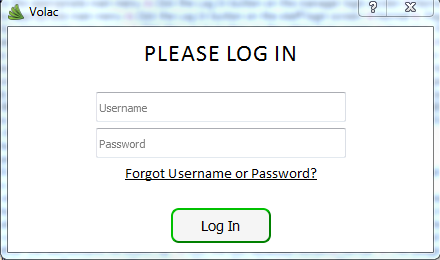
\includegraphics[width=\textwidth]{./Testing/Images/LoginScreen.png}
    \label{fig:LoginScreen}
\end{figure}

\begin{figure}[H]
    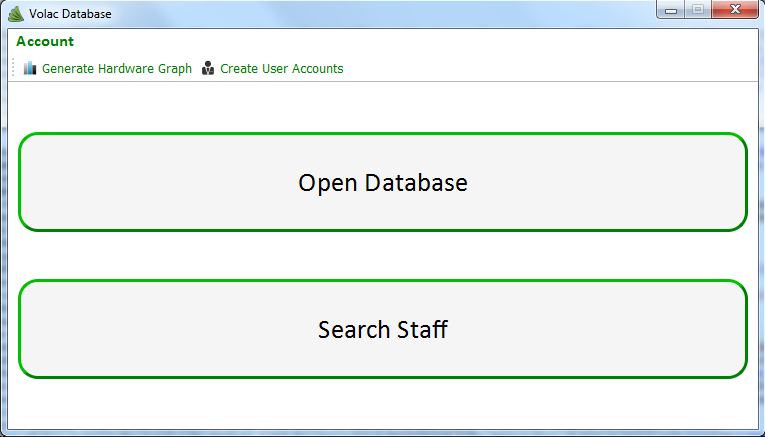
\includegraphics[width=\textwidth]{./Testing/Images/AdminInterface.png}
    \caption{This screen will be displayed if the user has logged in with Admin details.} \label{fig:AdminInterfaceLogin}
\end{figure}

\begin{figure}[H]
    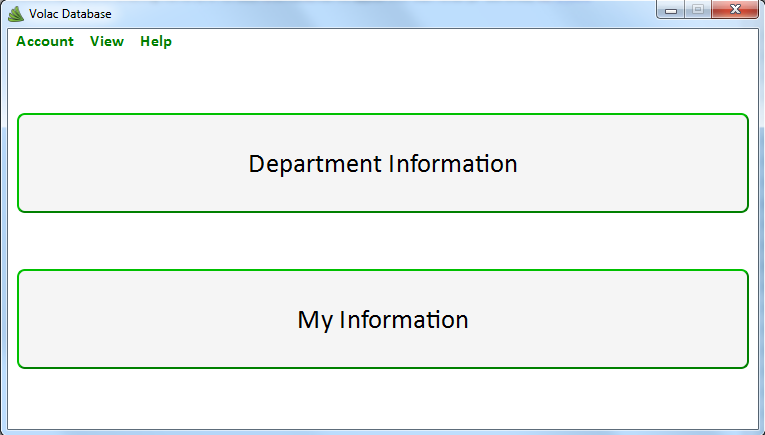
\includegraphics[width=\textwidth]{./Testing/Images/ManagerLogin.png}
    \caption{This screen will be displayed if the user has logged in with Manager details.} \label{fig:ManagerInterfaceLogin}
\end{figure}

\begin{figure}[H]
    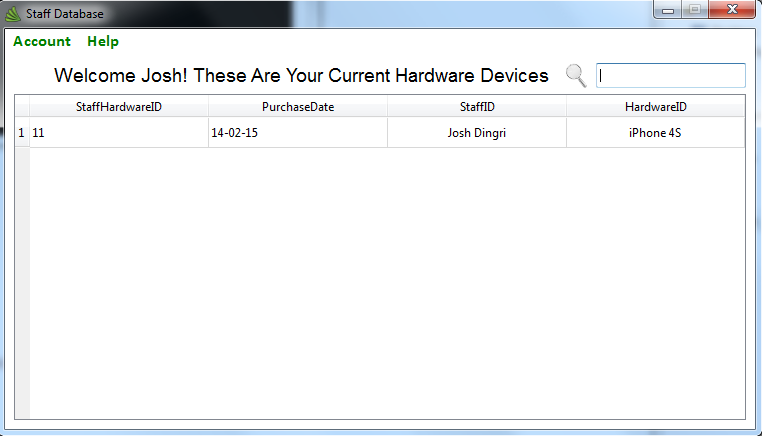
\includegraphics[width=\textwidth]{./Testing/Images/StaffLogin.png}
    \caption{This screen will be displayed if the user has logged in with Staff details.} \label{fig:StaffInterfaceLogin}
\end{figure}

\begin{figure}[H]
    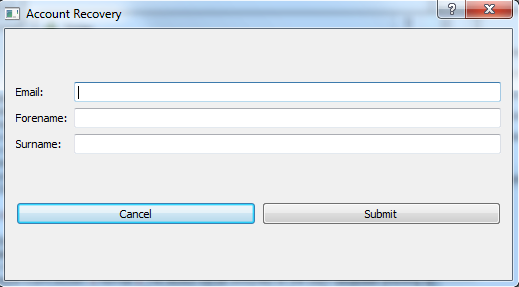
\includegraphics[width=\textwidth]{./Testing/Images/ForgotPassword.png}
    \caption{If the user presses the forgot username or password button this window will appear.} \label{fig:ForgotPassword}
\end{figure}

\begin{figure}[H]
    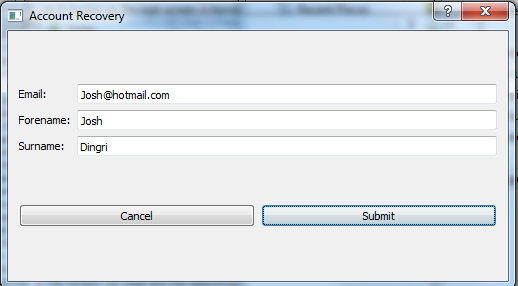
\includegraphics[width=\textwidth]{./Testing/Images/SubmitPassword.png}
    \caption{The user will fill out the details needed. After the submit button is pressed these details will be emailed to IT staff} \label{fig:SubmitPassword}
\end{figure}

\begin{figure}[H]
    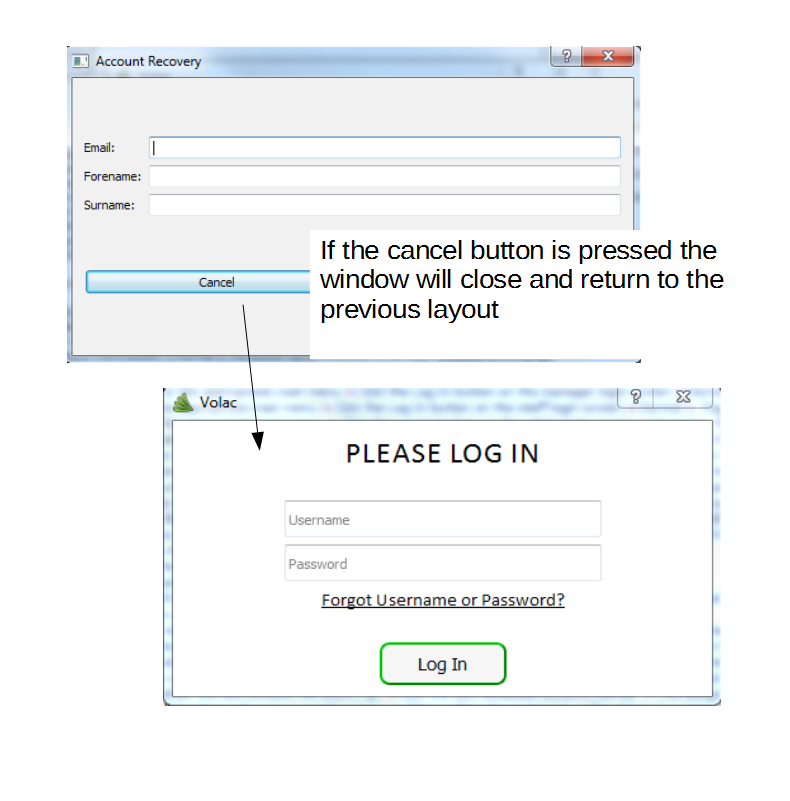
\includegraphics[width=\textwidth]{./Testing/Images/FogottenPasswordClose.png}
     \label{fig:FogottenPasswordClose}
\end{figure}

\begin{figure}[H]
    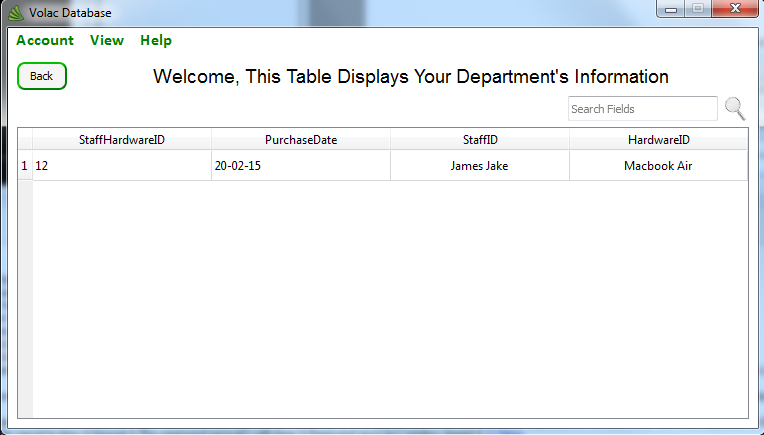
\includegraphics[width=\textwidth]{./Testing/Images/DepartmentInformation.png}
    \caption{The department information interface will appear when the button is clicked shown on the manager's home screen. \ref{fig:ManagerInterfaceLogin} } \label{fig:DepartmentInformation}
\end{figure}

\begin{figure}[H]
    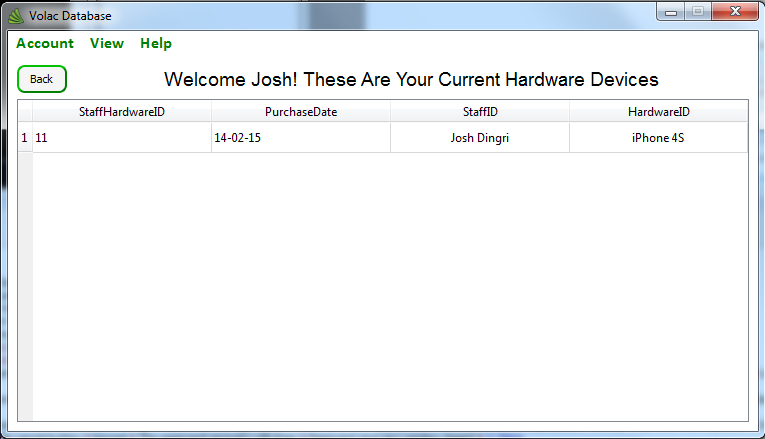
\includegraphics[width=\textwidth]{./Testing/Images/MyInformation.png}
    \caption{The my information interface will appear when the button is clicked shown on the manager's home screen. \ref{fig:ManagerInterfaceLogin} } \label{fig:MyInformation}
\end{figure}

\begin{figure}[H]
    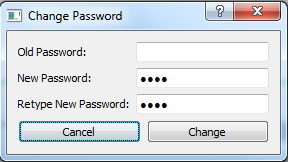
\includegraphics[width=100mm,scale=1]{./Testing/Images/ChangePasswordWindow.png}
    \caption{This is before the password is changed - After: \ref{fig:PassChange}} \label{fig:ChangePasswordWindow}
\end{figure}

\begin{figure}[H]
    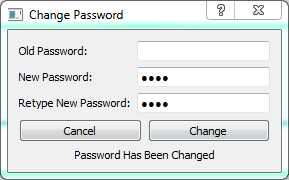
\includegraphics[width=100mm,scale=1]{./Testing/Images/PassChange1.png}
    \caption{This is after the password has been changed} \label{fig:PassChange}
\end{figure}

\begin{figure}[H]
    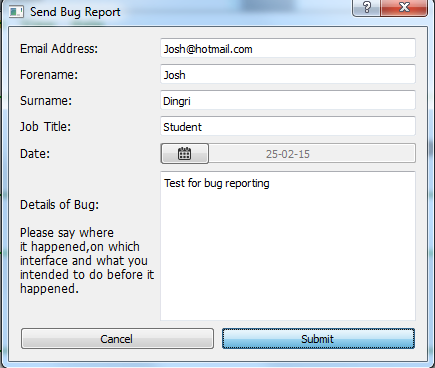
\includegraphics[width=\textwidth]{./Testing/Images/SubmitBugTest.png}
    \caption{When the submit button is pressed an email will be sent to IT staff with the above information.} \label{fig:SubmitBugTest}
\end{figure}

\begin{figure}[H]
    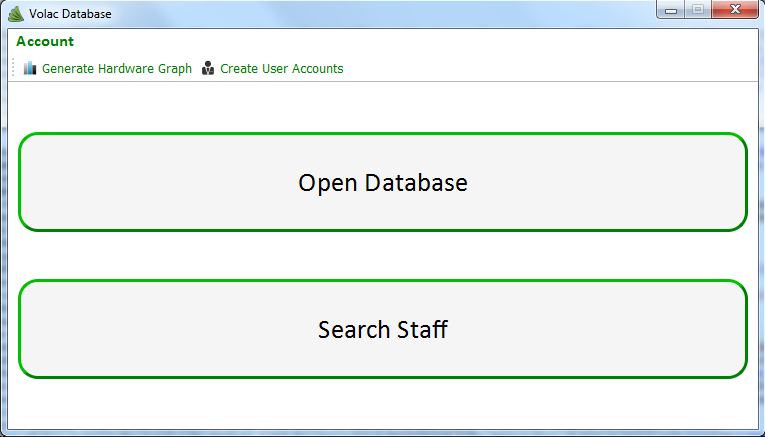
\includegraphics[width=\textwidth]{./Testing/Images/AdminInterface.png}
    \caption{Before the open database button is pressed - After: \ref{fig:OpenDatabaseInterface}} \label{fig:OpenDatabaseInterfaceBF}
\end{figure}


\begin{figure}[H]
    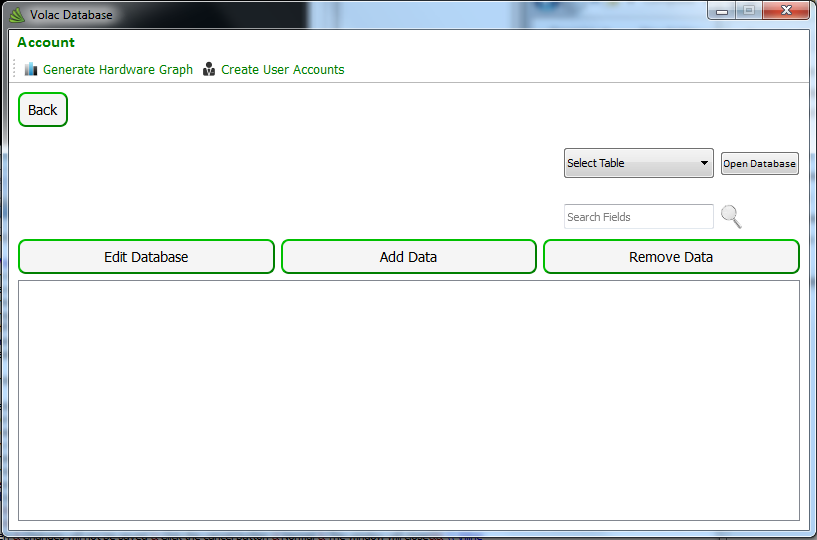
\includegraphics[width=\textwidth]{./Testing/Images/OpenDatabaseInterface.png}
    \caption{After the open database button is pressed the following interface will show.} \label{fig:OpenDatabaseInterface}
\end{figure}

\begin{figure}[H]
    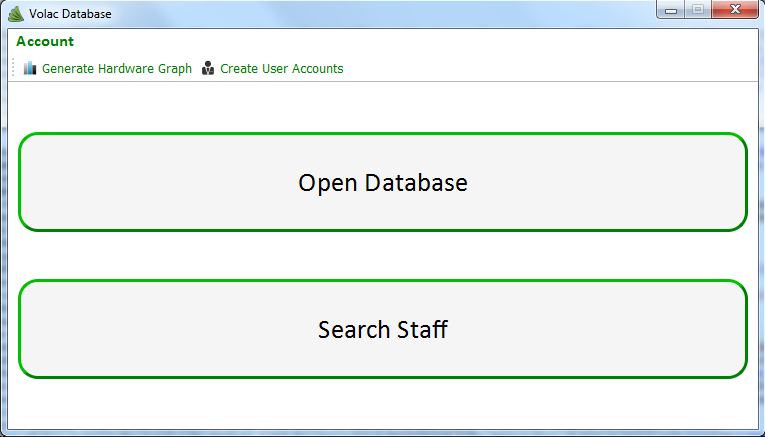
\includegraphics[width=\textwidth]{./Testing/Images/AdminInterface.png}
    \caption{Before the search staff button is pressed - After:\ref{fig:SearchStaffInterface}} \label{fig:SearchStaffInterfaceBF}
\end{figure}

\begin{figure}[H]
    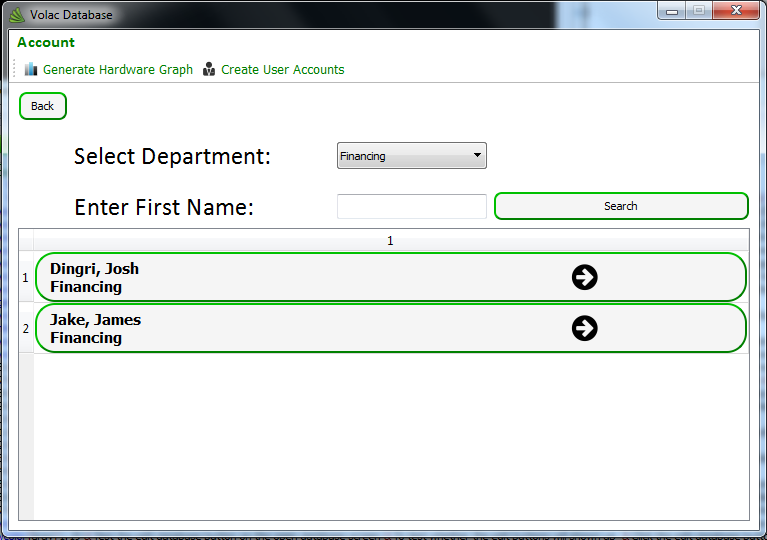
\includegraphics[width=\textwidth]{./Testing/Images/SearchStaffInterface.png}
    \caption{After the search staff button is pressed} \label{fig:SearchStaffInterface}
\end{figure}

\begin{figure}[H]
    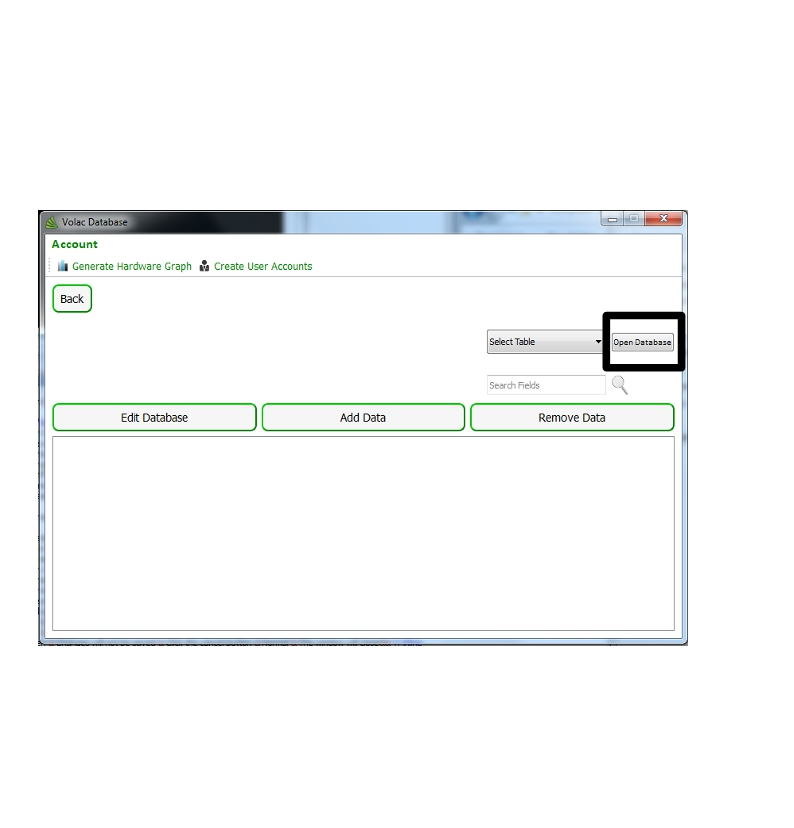
\includegraphics[width=\textwidth]{./Testing/Images/OpenDatabaseFileBefore.png}
    \caption{The user will click this button in order to open the database file. Next Image: \ref{fig:OpenDatabaseFileBrowser} } \label{fig:OpenDatabaseFileBefore}
\end{figure}

\begin{figure}[H]
    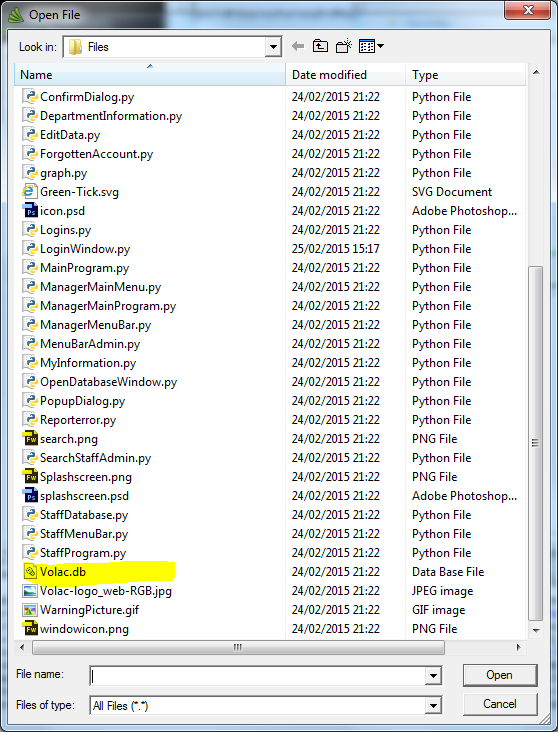
\includegraphics[width=\textwidth]{./Testing/Images/OpenDatabaseFileBrowser.png}
    \caption{The user should select the highlighted file above. Then click the open button. Next Image: \ref{fig:OpenDatabaseAfterBrowser}} \label{fig:OpenDatabaseFileBrowser}
\end{figure}


\begin{figure}[H]
    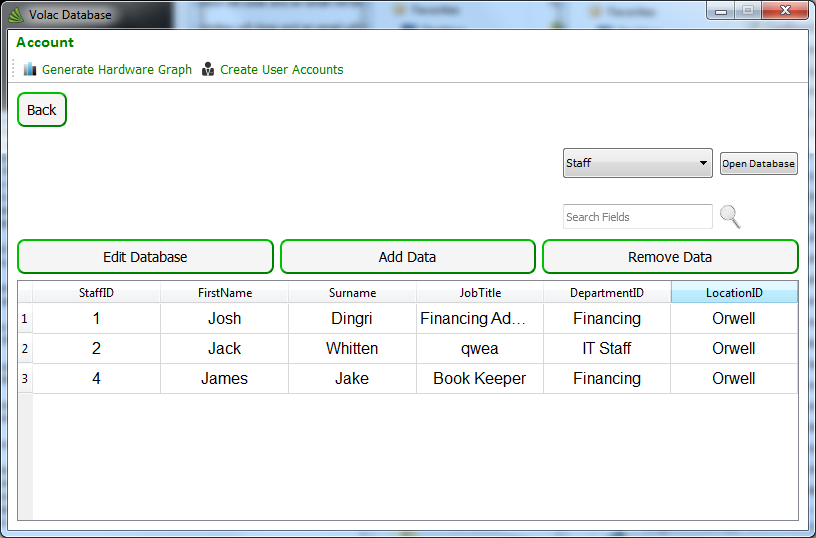
\includegraphics[width=\textwidth]{./Testing/Images/OpenDatabaseAfterBrowser.png}
    \caption{The database will open and the user can select a table using the combobox} \label{fig:OpenDatabaseAfterBrowser}
\end{figure}

\begin{figure}[H]
    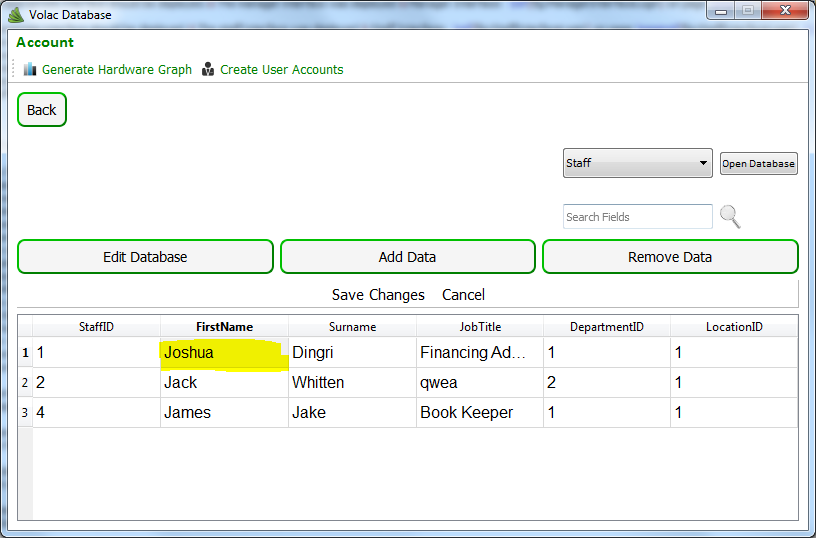
\includegraphics[width=\textwidth]{./Testing/Images/EditDataBtn.png}
    \caption{The above screenshot shows how the data can be edited if the user clicks the Edit Database button.} \label{fig:EditDataBtn}
\end{figure}

\begin{figure}[H]
    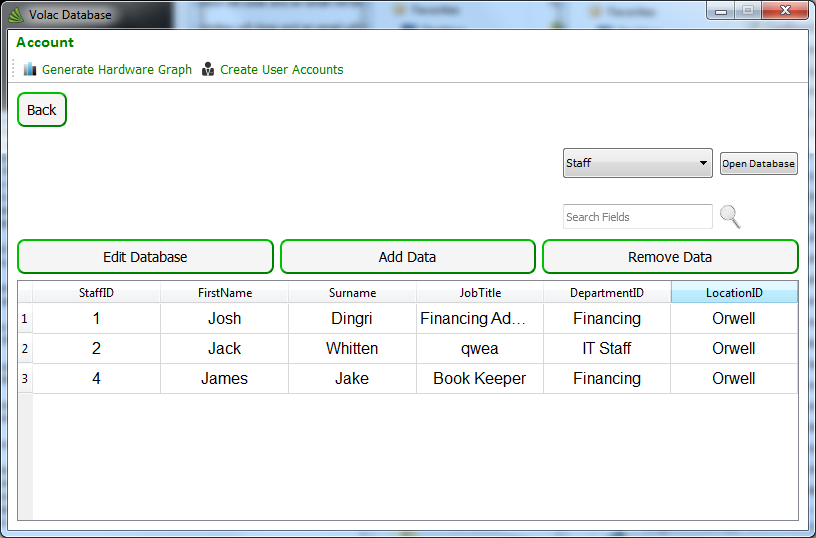
\includegraphics[width=\textwidth]{./Testing/Images/OpenDatabaseAfterBrowser.png}
    \caption{If the cancel button is pressed the data will return to normal.} \label{fig:CancelBtn}
\end{figure}

\begin{figure}[H]
    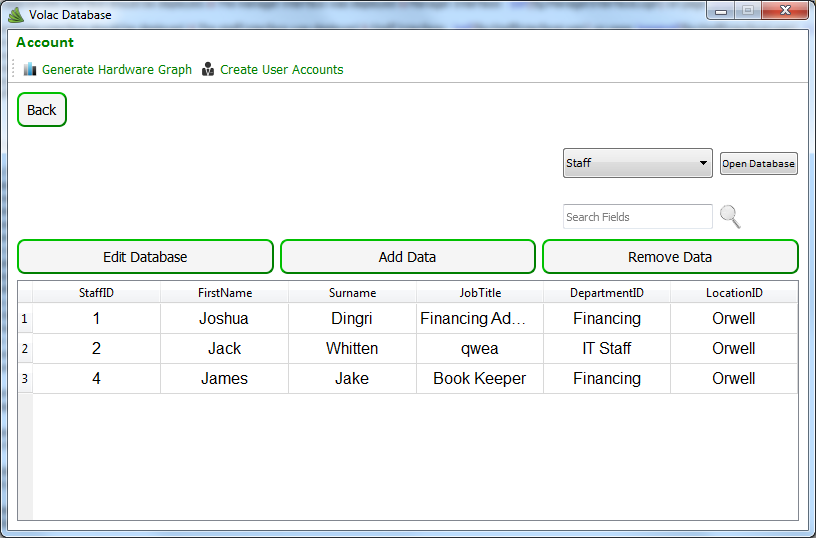
\includegraphics[width=\textwidth]{./Testing/Images/SaveChanges.png}
    \caption{The data is saved into the table and database if the save changes button is clicked.} \label{fig:SaveChanges}
\end{figure}

\begin{figure}[H]
    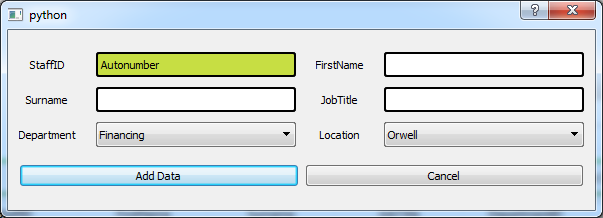
\includegraphics[width=\textwidth]{./Testing/Images/AddDataWindow.png}
    \caption{The window above will open if the user clicks add data.} \label{fig:AddDataWindow}
\end{figure}

\begin{figure}[H]
    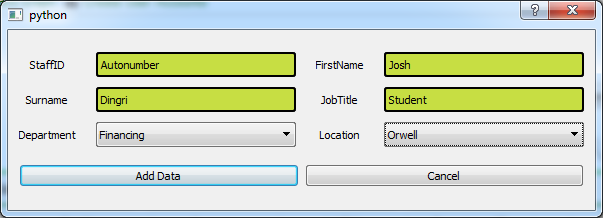
\includegraphics[width=\textwidth]{./Testing/Images/AddDataDataExample.png}
    \caption{The user will fill out all the necessary data shown above and then will click the add data button. Next Image: \ref{fig:AddedData}} \label{fig:AddDataDataExample}
\end{figure}

\begin{figure}[H]
    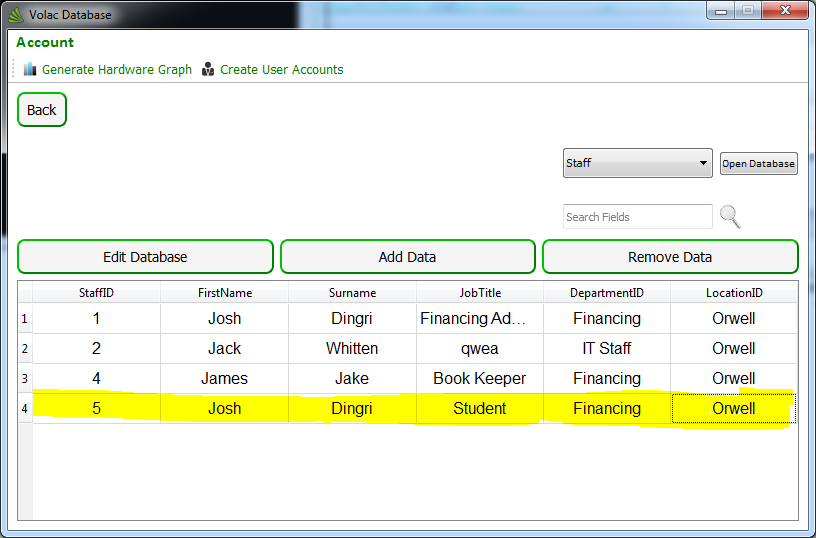
\includegraphics[width=\textwidth]{./Testing/Images/AddedData.png}
    \caption{The data is added to the table and database} \label{fig:AddedData}
\end{figure}

\begin{figure}[H]
    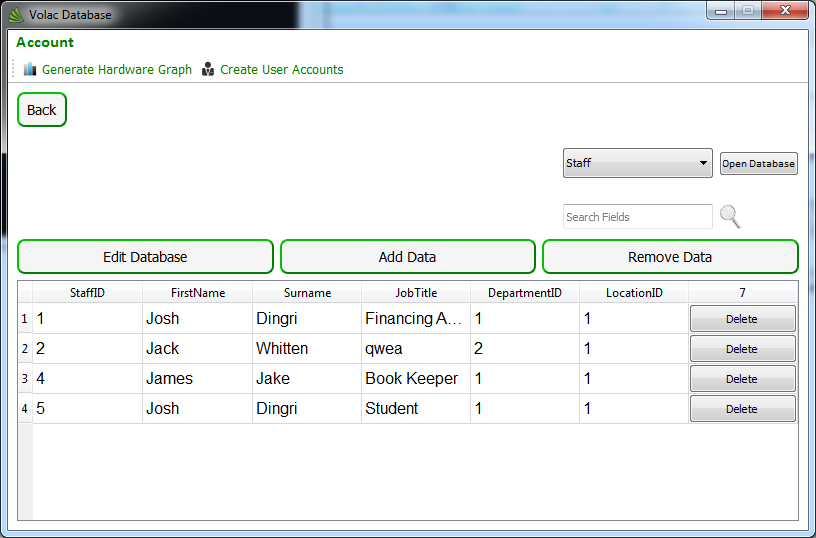
\includegraphics[width=\textwidth]{./Testing/Images/RemoveDataButtons.png}
    \caption{When the remove data button is clicked the delete buttons will appear to allow the user to remove records. Next Image: \ref{fig:NoButton}} \label{fig:RemoveDataButtons}
\end{figure}


\begin{figure}[H]
    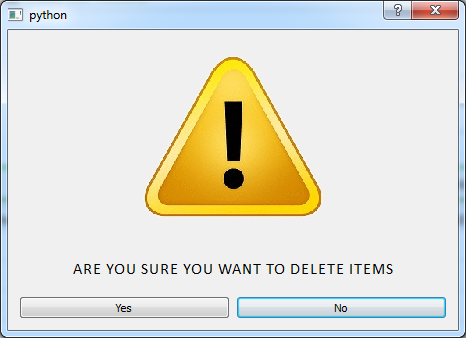
\includegraphics[width=\textwidth]{./Testing/Images/NoButton.png}
    \caption{If the no button is clicked on the warning window the data will be kept and the window will close} \label{fig:NoButton}
\end{figure}

\begin{figure}[H]
    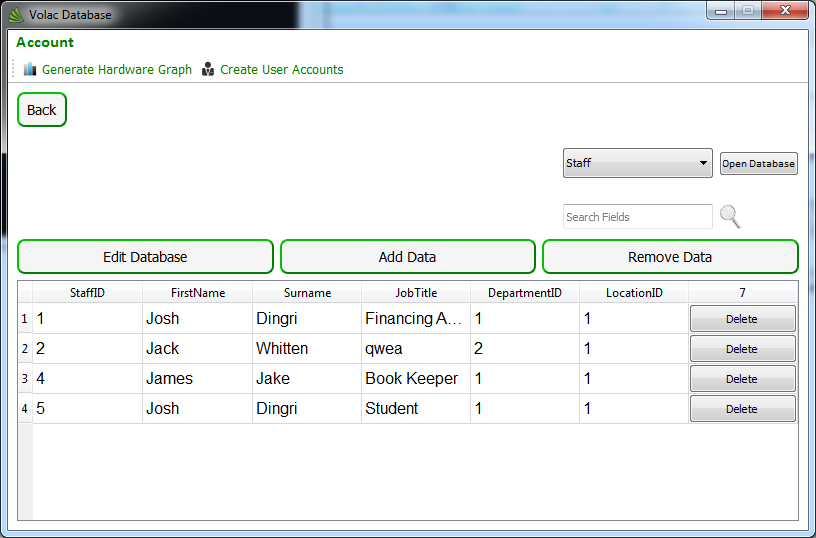
\includegraphics[width=\textwidth]{./Testing/Images/RemoveDataButtons.png}
    \caption{Data is kept}
\end{figure}

\begin{figure}[H]
    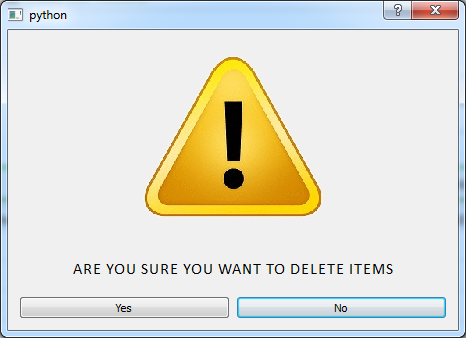
\includegraphics[width=\textwidth]{./Testing/Images/NoButton.png}
    \caption{If the yes button is clicked on the warning window the data will be removed and the window will close. Next Image: \ref{fig:RemovedData}} \label{fig:YesBtn}
\end{figure}

\begin{figure}[H]
    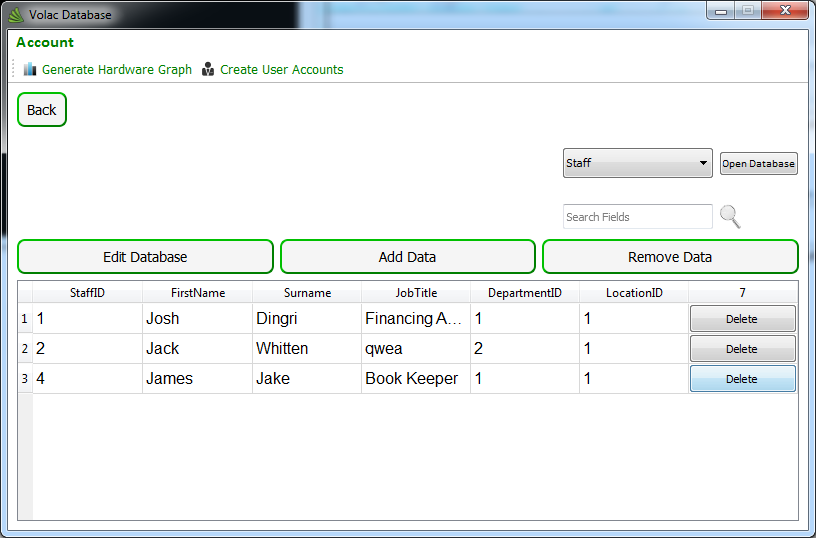
\includegraphics[width=\textwidth]{./Testing/Images/RemovedData.png}
    \caption{Data is removed} \label{fig:RemovedData}
\end{figure}

\begin{figure}[H]
    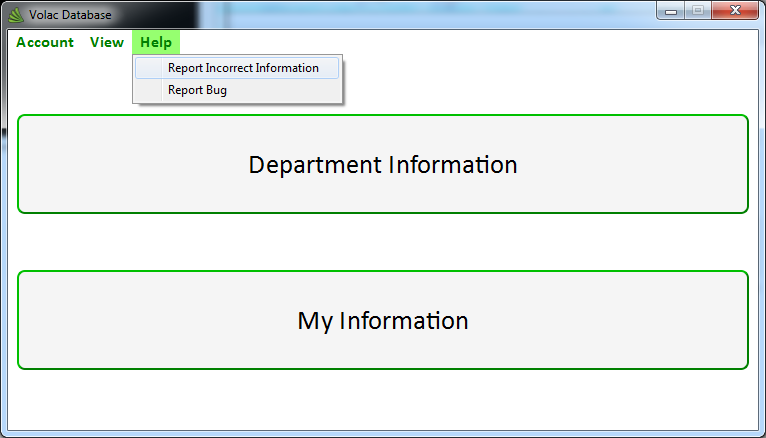
\includegraphics[width=\textwidth]{./Testing/Images/HelpMenu.png}
    \caption{Screenshot showing that the help menu works as expected} \label{fig:HelpMenu}
\end{figure}

\begin{figure}[H]
    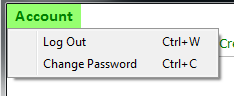
\includegraphics[width=\textwidth]{./Testing/Images/AccountMenu.png}
    \caption{Screenshot showing that the account menu works as expected} \label{fig:AccountMenu}
\end{figure}

\begin{figure}[H]
    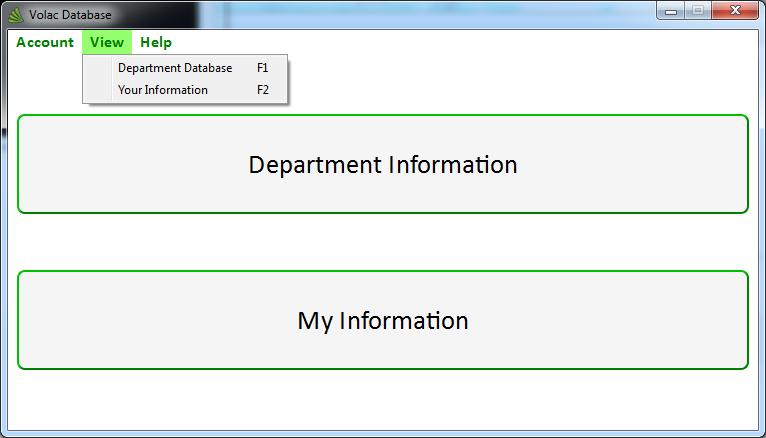
\includegraphics[width=\textwidth]{./Testing/Images/ViewMenu.png}
    \caption{Screenshot showing that the view menu works as expected} \label{fig:ViewMenu}
\end{figure}


\begin{figure}[H]
    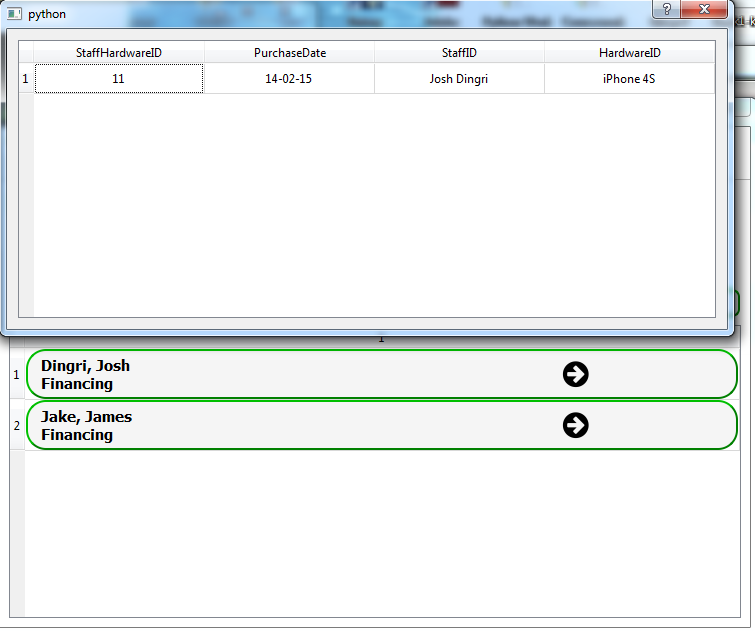
\includegraphics[width=\textwidth]{./Testing/Images/SearchStaffButtons.png}
    \caption{If a button is clicked the window showing more information will show up.} \label{fig:SearchStaffButtons}
\end{figure}

\begin{figure}[H]
    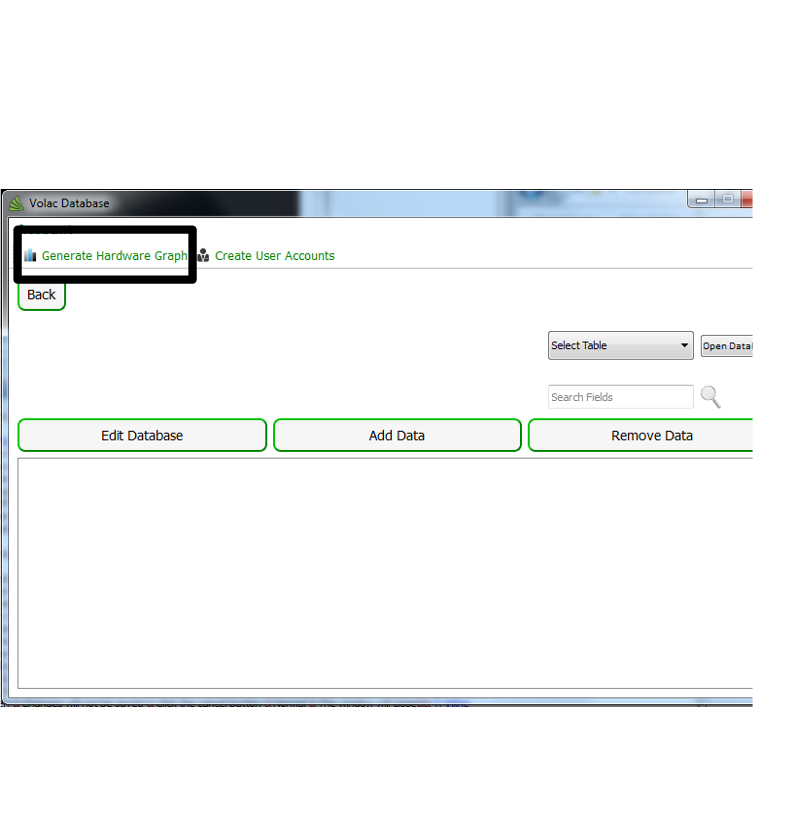
\includegraphics[width=\textwidth]{./Testing/Images/OpenGraphBtn.png}
    \caption{Before the graph button is pressed. Next Image: \ref{fig:GraphButton}} \label{fig:GraphBtn}
\end{figure}

\begin{figure}[H]
    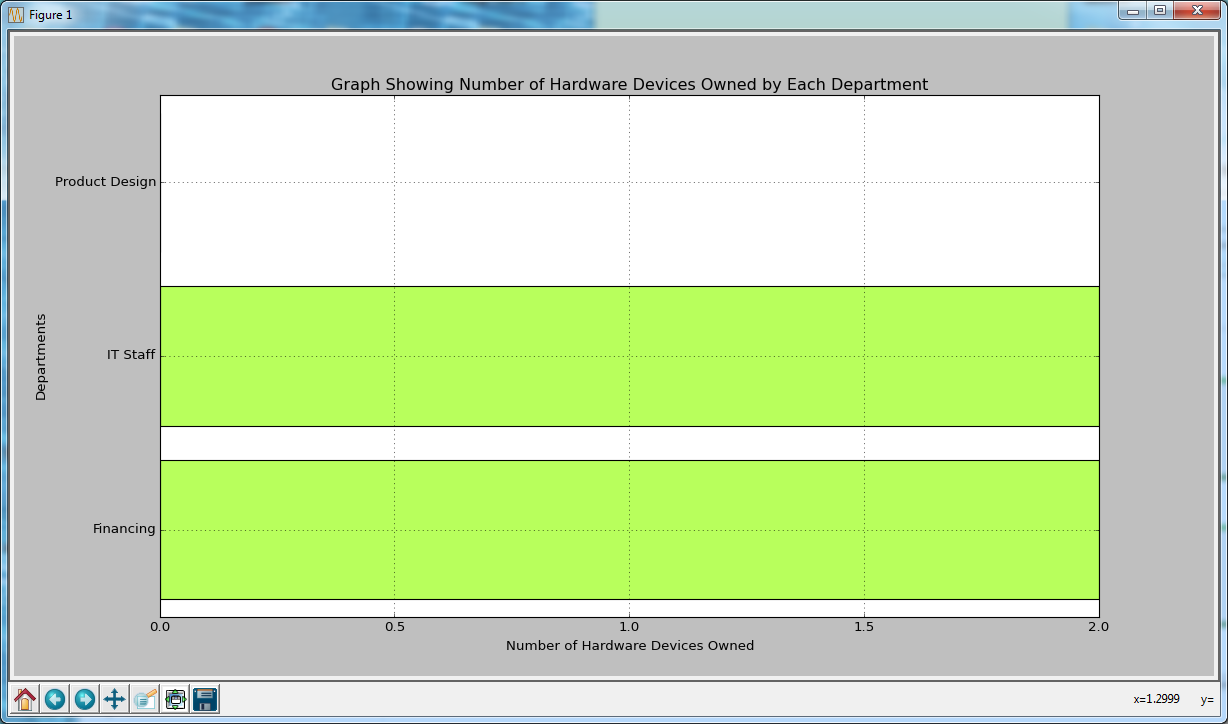
\includegraphics[width=\textwidth]{./Testing/Images/GraphButton.png}
    \caption{After the graph button is pressed} \label{fig:GraphButton}
\end{figure}

\begin{figure}[H]
    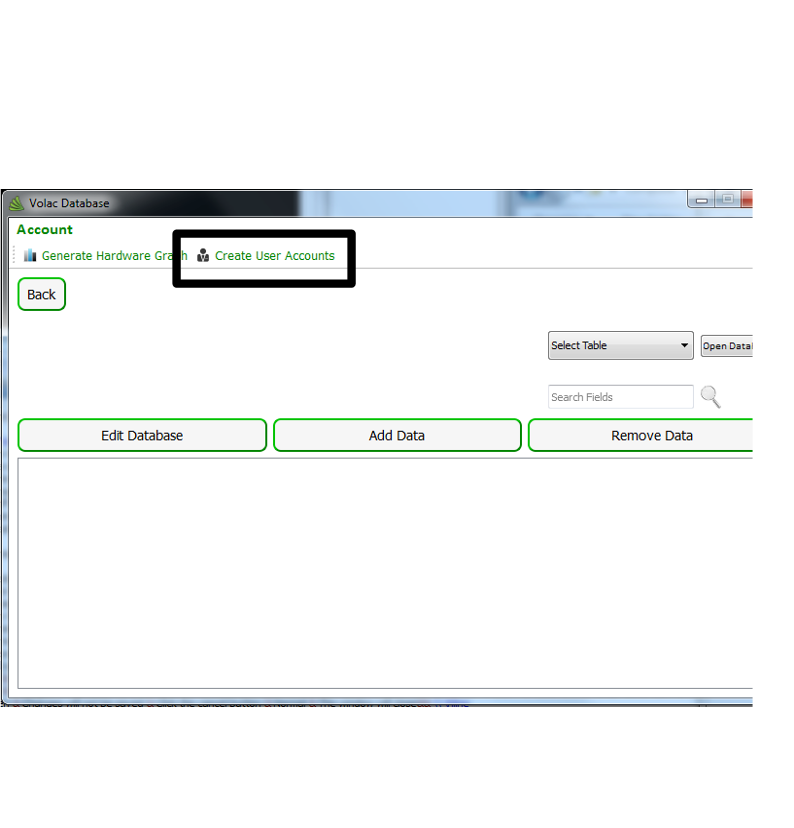
\includegraphics[width=\textwidth]{./Testing/Images/AddAccountBtn.png}
    \caption{Before the create account is pressed - Next Image: \ref{fig:AddAccountsButton}} \label{fig:AddAccountsBtn}
\end{figure}

\begin{figure}[H]
    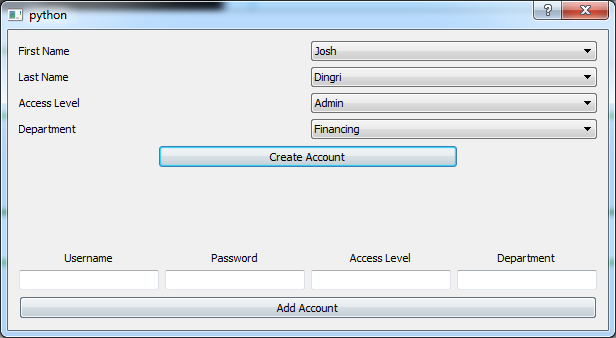
\includegraphics[width=\textwidth]{./Testing/Images/AddAccountsButton.png}
    \caption{After the create account is pressed - Next Image: \ref{fig:AddAccountDetails}} \label{fig:AddAccountsButton}
\end{figure}

\begin{figure}[H]
    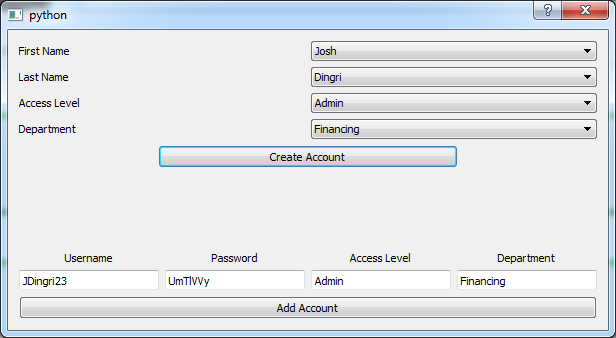
\includegraphics[width=\textwidth]{./Testing/Images/AddAccountDetails.png}
    \caption{After the create account button is clicked the line edits will automatically fill} \label{fig:AddAccountDetails}
\end{figure}

\begin{figure}[H]
    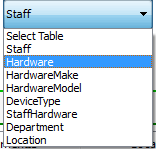
\includegraphics[width=50mm,scale=0.5]{./Testing/Images/ComboBoxHardware.png}
    \caption{Example of dropdown box on open database interface to choose table.} \label{fig:ComboBoxHardware}
\end{figure}

\begin{figure}[H]
    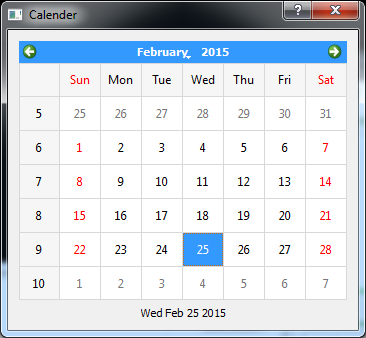
\includegraphics[width=\textwidth]{./Testing/Images/Calendar.png}
    \caption{When the calendar button is clicked on the add data window. Next Image: \ref{fig:CalendarAdd}} \label{fig:Calendar}
\end{figure}

\begin{figure}[H]
    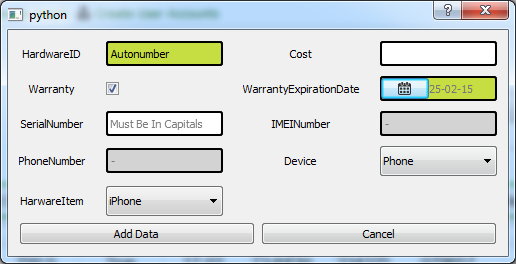
\includegraphics[width=\textwidth]{./Testing/Images/CalendarAddData.png}
    \caption{After the date has been selected it will appear in the line edit next to the button} \label{fig:CalendarAdd}
\end{figure}

\begin{figure}[H]
    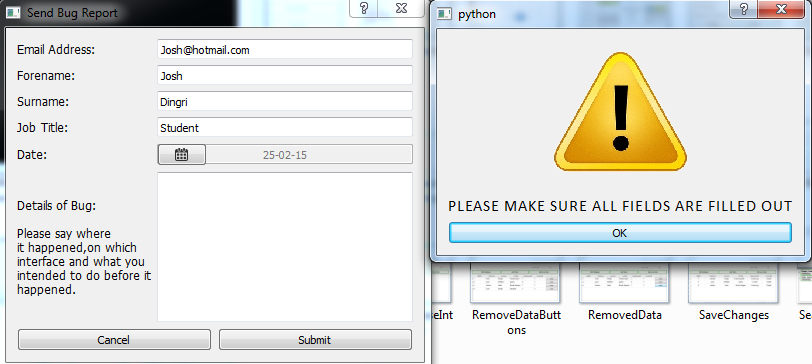
\includegraphics[width=\textwidth]{./Testing/Images/ReportBugValidation.png}
    \caption{Warning window appears if not all fields have been completed} \label{fig:ReportBugValidation}
\end{figure}

\begin{figure}[H]
    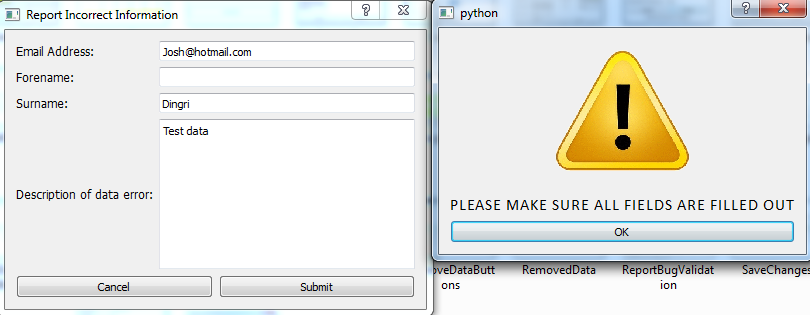
\includegraphics[width=\textwidth]{./Testing/Images/ReportErrorValidation.png}
    \caption{Warning window appears if not all fields have been completed} \label{fig:ReportErrorValidation}
\end{figure}

\begin{figure}[H]
    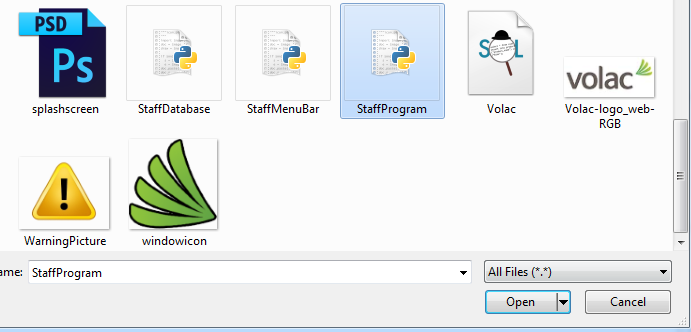
\includegraphics[width=\textwidth]{./Testing/Images/IncorrectFile.png}
    \caption{The screenshot shows someone selecting the incorrect file. Next Image: \ref{fig:IncorrectFileError}} \label{fig:IncorrectFile}
\end{figure}

\begin{figure}[H]
    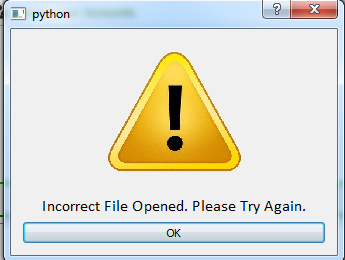
\includegraphics[width=80mm,scale=0.5]{./Testing/Images/IncorrectFileError.png}
    \caption{The screenshot shows the warning that will appear if the incorrect file is opened} \label{fig:IncorrectFileError}
\end{figure}

\begin{figure}[H]
    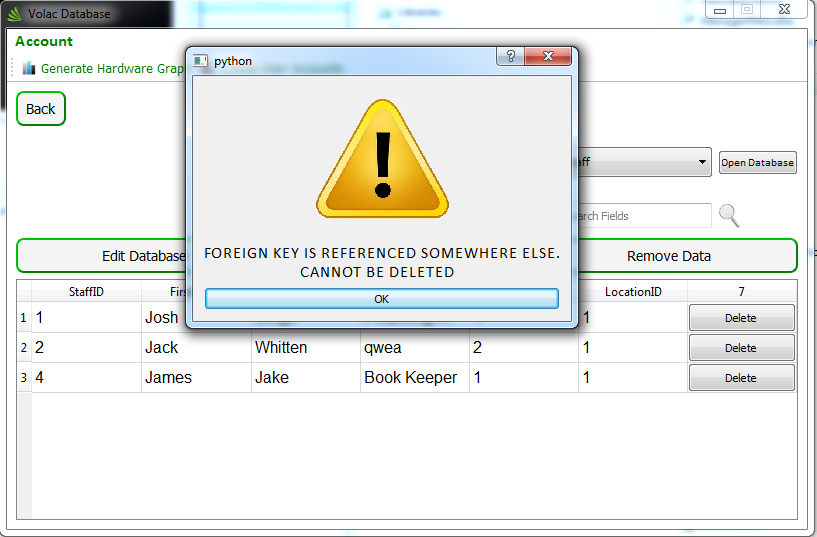
\includegraphics[width=\textwidth]{./Testing/Images/DialogNoClickAway.png}
    \caption{If a user attempts to delete a primary key that is referenced somewhere else this error will appear and the user will not be able to remove it until the foreign keys that reference have been deleted.} \label{fig:DialogNoClickAway}
\end{figure}

\begin{figure}[H]
    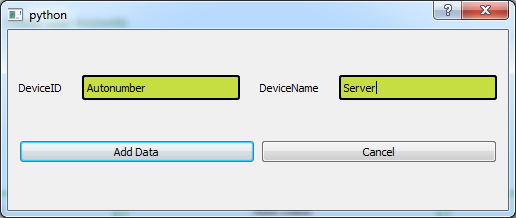
\includegraphics[width=\textwidth]{./Testing/Images/Dev.png}
    \caption{A device being added to the device type table. Next Image: \ref{fig:AddedDevice}} \label{fig:Dev}
\end{figure}

\begin{figure}[H]
    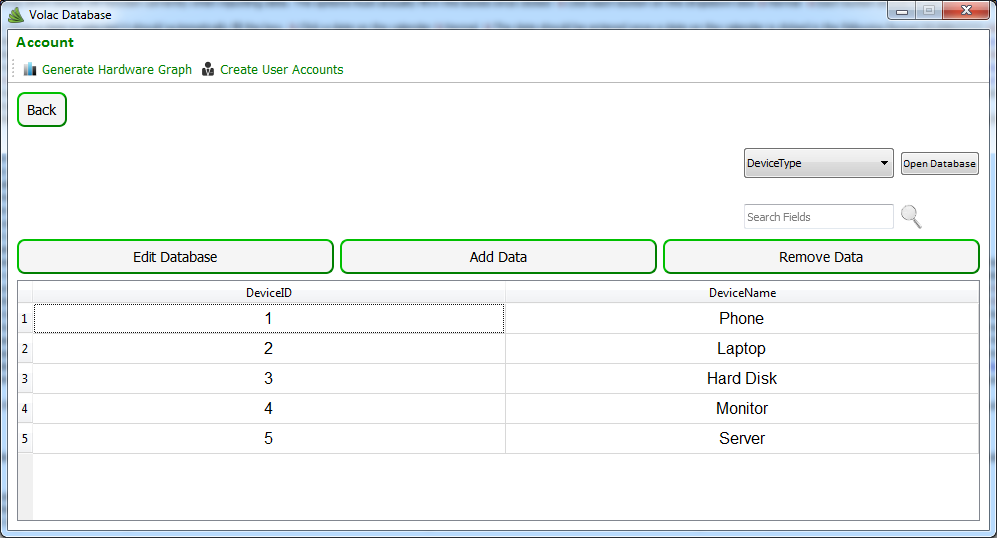
\includegraphics[width=\textwidth]{./Testing/Images/AddedDevice.png}
    \caption{The device will then appear correctly in the table (and added to the database)} \label{fig:AddedDevice}
\end{figure}


\begin{figure}[H]
    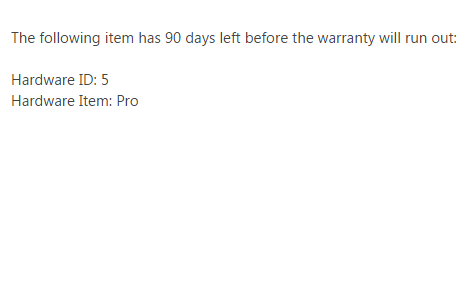
\includegraphics[width=\textwidth]{./Testing/Images/EmailExpiredHardware.png}
    \caption{This email example shows how the automatic warranty email will look in the email inbox.} \label{fig:EmailExpiredHardware}
\end{figure}


\begin{figure}[H]
    \includegraphics[width=\textwidth]{./Testing/Images/DepartmentInformationButton.png}
    \caption{The F1 and F2 shortcuts shown and working.} \label{fig:DepartmentInformationButton}
\end{figure}

\begin{figure}[H]
    \includegraphics[width=\textwidth]{./Testing/Images/BeforeSearch.png}
    \caption{Before the search button has been pressed and the program shows all staff in the department selected  Next Image: \ref{fig:AfterSearch}} \label{fig:BeforeSearch}
\end{figure}

\begin{figure}[H]
    \includegraphics[width=\textwidth]{./Testing/Images/AfterSearch.png}
    \caption{After the search button has been pressed and the program narrows to search} \label{fig:AfterSearch}
\end{figure}

\begin{figure}[H]
    \includegraphics[width=\textwidth]{./Testing/Images/ChangedPassword.png}
    \caption{The password has been changed from nothing to 'qwerty'  Next Image: \ref{fig:ChangedPasswordOld}} \label{fig:ChangedPassword}
\end{figure}

\begin{figure}[H]
    \includegraphics[width=\textwidth]{./Testing/Images/ChangedPasswordOld.png}
    \caption{The user can now not login with no password  Next Image: \ref{fig:ChangePasswordNew}} \label{fig:ChangedPasswordOld}
\end{figure}

\begin{figure}[H]
    \includegraphics[width=\textwidth]{./Testing/Images/ChangePasswordNew.png}
    \caption{The user can log in with 'qwerty' Next Image: \ref{fig:AdminNewPassword}} \label{fig:ChangePasswordNew}
\end{figure}

\begin{figure}[H]
    \includegraphics[width=\textwidth]{./Testing/Images/AdminInterface.png}\label{fig:AdminNewPassword}
\end{figure}

\begin{figure}[H]
    \includegraphics[width=\textwidth]{./Testing/Images/ManagerNoChange.png}
    \caption{The user cannot change any information. It is in read only format. Next Image: \ref{fig:StaffNoChange}} \label{fig:ManagerNoChange}
\end{figure}

\begin{figure}[H]
    \includegraphics[width=\textwidth]{./Testing/Images/StaffNoChange.png}
    \caption{The user cannot change any information. It is in read only format.} \label{fig:StaffNoChange}
\end{figure}

\begin{figure}[H]
    \includegraphics[width=60mm,scale=0.5]{./Testing/Images/CurrentDate.png}
    \caption{The current date shown for proof of email Next Image: \ref{fig:HardwareDate}} \label{fig:CurrentDate}
\end{figure}

\begin{figure}[H]
    \includegraphics[width=\textwidth]{./Testing/Images/HardwareDate.png}
    \caption{Date showing 90 days in the future to test the email Next Image: \ref{fig:EmailExpiredHardware}} \label{fig:HardwareDate}
\end{figure}

\begin{figure}[H]
    \includegraphics[width=\textwidth]{./Testing/Images/EmailExpiredHardware.png}
    \caption{Email comes through referencing hardware item.} \label{fig:EmailExpiredHardware}
\end{figure}




\section{Evaluation}

\subsection{Approach to Testing}

I used decided to use a wide range of testing strategies to look out the different aspects of the program. For example to test the GUI in series 1 top-down testing was performed to check the if all the interfaces and the flow between them was working correctly. Bottom-up testing was used in series 2 to test the validation were functioning correctly, it was also used in series 4 to check the data can be read through the tables from the database file. Black-box testing was used in series 3 to make sure that the data was in fact being stored in the database and that emails were sent and stored in inboxes. Black-box testing was also used in series 7 to check shortcuts were working correctly. Unit testing was used in series 5 to test the different main programs for Staff, Managers and Admins on different access levels. Acceptance testing was used for series 6 to make sure the whole system worked correctly and met the specifications I compared this test with my original objectives.

\subsection{Problems Encountered}

The testing allowed me to see problems in my system. For example in test 6 the system actually didn't meet the full specifications that the client wanted. The amount of time I had was just enough to produce the GUI for the system I did not have the time or skill needed to produce an online version so multiple staff can access it at once. However I can add this functionality to my system at a later date. Also when editing and removing data the system removed the text foreign keys are reverts to numbers to reference primary keys, obviously this is a very unfriendly way to delete and edit data ( \ref{fig:RemoveDataButtons}).

\par Another issue was in test 8.4. The problem here was with the automated email. It does not work in the way that is ideal since it will not automatically work out dates while the program is running, instead it can only work out the days left if the program is restarted once a day. However most likely the program would be reset each day in a real company, but it is still a big problem that would need to be fixed at a later date.

\subsection{Strengths of Testing}

The strengths of my testing came from the wide range of testing I did. Mainlythis was from the GUI with top-down testing in series 1. I covered my whole system and uncovered any problems shown above. In series 3 I also managed to perform a lot of validation tests covering the entire system which made sure any user can use the system without running into any errors.

\subsection{Weaknesses of Testing}

My weakness was mostly around test series 8 when testing algorithms. There were a lot more than just this amount of algoritms in the system and it may have been useful to identiify them.

\subsection{Reliability of Application}

Reliability when relating to my system is used to explain if it is consistently performing according to its specifications. I believe that testing has shown that my system is largly reliable as it thoroughly tests my whole system and outlines where the problems are, however there are only a few of problems in the entire system (that have been found - 6 and 8.4) which proves its reliability. The main problem that effects reliability that can be fixed is the fact that foreign keys arent user friendly when removing or editing data.

\subsection{Robustness of Application}

Robustness is used when explaining if the software can cope with any errors during execution. The testing has proved that my program handles errors very well. At no point was an error shown in the console and all calculations were made correctly. Any errors were shown with a GUI error message to allow the user of the system understand what they have done wrong.
